% see http://info.semprag.org/basics for a full description of this template
\documentclass[cm]{glossa}
% possible options: 
% [times] for Times font (default if no option is chosen)
% [cm] for Computer Modern font 
% [lucida] for Lucida font (not freely available)
% [brill] open type font, freely downloadable for non-commercial use from http://www.brill.com/about/brill-fonts; requires xetex
% [charis] for CharisSIL font, freely downloadable from http://software.sil.org/charis/
% for the Brill an CharisSIL fonts, you have to use the XeLatex typesetting engine (not pdfLatex)
% [biblatex] for using biblatex
% [linguex] loads the linguex example package
% !! a note on the use of linguex: in glossed examples, the third line of the example (the translation) needs to be prefixed with \glt. This is to allow a first line with the name of the language and the source of the example. See example (2) in the text for an illustration.
% !! a note on the use of bibtex: for PhD dissertations to typeset correctly in the references list, the Address field needs to contain the city (for US cities in the format "Santa Cruz, CA")

%\addbibresource{sample.bib} % this is for use with biblatex; replace this by the name of your bib-file (extension .bib is required); comment out if you use natbib

\usepackage{sectsty} %control style of section headings
\allsectionsfont{\normalfont\sffamily\bfseries} %sans serif boldface in section headings
\let\B\relax %to resolve a conflict in the definition of these commands between xyling and xunicode (the latter called by fontspec, called by charis)
\let\T\relax
%\usepackage{xyling} %for trees; the use of xyling with the CharisSIL font produces poor results in the branches. This problem does not arise with the packages qtree or forest.
\usepackage{forest} %for nice trees!
\usepackage{booktabs} % for tables
\usepackage{multirow}
\usepackage{qtree} % trees
\qtreecenterfalse
\usepackage{tree-dvips}
% \usepackage{qdotbranch}
%\usepackage{xeCJK} % Chinese characters
%\setCJKmainfont{SimSun}
\usepackage{linguex} % must come after xeCJK
%\usepackage{tree-dvips}
% \usepackage{underarrows}

\newcommand{\sem}[1]{\mbox{$[\![$#1$]\!]$}}
\newcommand{\type}[1]{\ensuremath{\left \langle #1 \right \rangle }}
\newcommand{\lam}{\ensuremath{\lambda}}
\renewcommand{\and}{$\wedge$ }

\newcommand{\gcs}[1]{\textcolor{blue}{[gcs: #1]}} 
\newcommand{\lsp}[1]{\textcolor{red}{[lsp: #1]}}
\newcommand{\lp}[1]{\textcolor{black}{#1}} % Lisa in-line edits

\renewcommand{\firstrefdash}{}


% \pdf* commands provide metadata for the PDF output. ASCII characters only!
\pdfauthor{Full author name}
\pdftitle{Full title}
\pdfkeywords{Full keyword list, separated, by, commas}

% Optional short title inside square brackets, for the running headers. If no short title is given, no title appears in the headers.

\title[When pragmatics matters more for truth-value judgments]{\lp{When} pragmatics \lp{matters more 
for} truth-value judgments: 
\lp{
%in acquisition investigations: \\
An investigation of quantifier scope ambiguity}}

% Optional short author inside square brackets, for the running headers. If no short author is given, no authors print in the headers.

% \author[Scontras \& Pearl]% short form of the author names for the running header
% {%as many authors as you like, each separated by \AND.
%   \spauthor{Gregory Scontras\\ 
%   \institute{University of California, Irvine}\\
%   \small{g.scontras@uci.edu}
%   }%
%   \AND
%   \spauthor{Lisa S.~Pearl \\
%   \institute{University of California, Irvine}\\
%   \small{lpearl@uci.edu}
%   }%
% }



\begin{document}

\sffamily
\maketitle


\begin{abstract}
% \lsp{I feel like we need to mention the case study that we're focusing on (i.e., quantifier scope ambiguity), even if we don't specifically mention the every-not sentences in the abstract. Of course, I'm a fan of concrete examples, so I'd actually be for mentioning an every-not sentence in the abstract. Similarly for the title---I'd feel better if we have something about the quantifier scope ambiguity in there too.}
Investigations of linguistic meaning rely crucially on truth-value judgments, which assess whether a sentence can truthfully describe a given scenario. \lp{In investigations of language acquisition, truth-value judgments are used to assess both the target knowledge adults have and the developing knowledge children have at different ages.} On the basis of \lp{truth-value judgments}, researchers have concluded that
\lp{differences between how children resolve ambiguous utterances and how adults do so persist until at least age five.}
%young children perform quite differently from adults when it comes to understanding ambiguous utterances with multiple potential meanings. 
% For example, when adults hear ``Every horse didn't jump over the fence,'' they entertain two interpretations: either none of the horses jumped or not all of the horses jumped. Children usually only endorse the ``none'' interpretation, rejecting the utterance in a scenario where only two out of three horses jumped. However, subtle changes to the truth-value judgment task setup make children more adult-like. We summarize key results from the literature on child ambiguity resolution, noting three core variables that affect children’s disambiguation behavior. One of these variables concerns children's processing ability: how easy it is to access the different grammatical interpretations. The other two variables concern children's ability to manage the pragmatic context: understanding what the topic of conversation is, and modulating expectations about the world being described.
\lp{Current explanations compatible with the experimental data attribute these differences to both grammatical processing and pragmatic factors.}
\lp{Here, we use computational cognitive modeling to formally articulate the ambiguity-resolution process that underlies child and adult judgments in a truth-value judgment task; crucially, the model can separate out the individual contributions of specific grammatical processing and pragmatic factors to the resulting judgment behavior.}
%We explore the nature of the truth-value judgment task children are being asked to engage in, which we then formally articulate using a cognitive computational model that specifies the role of various linguistic and extra-linguistic factors in providing truth-value judgments. 
%The results suggest that 
\lp{We find that}
pragmatic factors play a larger role than grammatical processing factors in explaining children's non-adult-like ambiguity resolution behavior, and the computational modeling framework allows us to understand exactly why that is.
%so. 
% \lp{Interestingly, our modeling results suggest that the truth-value judgment}
% %Indeed, by modeling the task itself, we see that the truth-value judgment 
% data typically used to demonstrate children's difficulty with ambiguity in fact require no disambiguation at all---just the ability to manage the pragmatics of the task,
% \lp{and children learn to get better at this as they become adults.}
\lp{Interestingly, the model predicts qualitative similarity between child and adult ambiguity resolution. Given this prediction,}
%In an extension of our model, 
we then 
\lp{extend our model to}
show how the same processes are active in adult 
\lp{ambiguity resolution.}
%language understanding, 
\lp{This result supports}
%thereby supporting the theory of 
continuity in the development of ambiguity resolution,
\lp{where children do not qualitatively change how they resolve ambiguity in order to become adult-like}.
\lp{We discuss the implications of our results for acquisition more generally, including both theories of development and
methods for assessing that development.
}
 
\end{abstract}

\begin{keywords}
truth-value judgments; ambiguity; development; pragmatics; Rational Speech Act model
\end{keywords}

% \end{frontmatter}

%\tableofcontents

\rmfamily

\section{Introduction}

% \lsp{Since we talk about meaning first in the paragraphs below, I thought we might reorder this opening bit to match.}
%How do our \lp{utterances} come to mean what they do, and how should we characterize that meaning? 
\lp{How should we characterize the meaning of sentences, and how do we (as speakers) learn that meaning?}
These questions call into focus the intersection of two traditions of inquiry: 
%language development and 
the semantics of natural language
\lp{and language development.}
One of the key empirical methodologies for questions at this intersection is the truth-value judgment 
% \lp{(\textbf{truth-value judgment})}
task \citep{crainmckee1985,crainthornton1998}. 
%The current work 
\lp{Here, we}
\lp{use a complementary methodology to investigate}
%bring a critical eye to 
%\lp{the truth-value judgment} methodology
%\lp{-- and importantly, 
\lp{how to interpret truth-value judgment behavior in specific cases where the truth-value judgment task has been used.}
\lp{More specifically, we}
model the cognitive processes, both linguistic and extra-linguistic, that deliver \lp{truth-value judgment} task behavior \lp{in precise experimental contexts}.
\lp{This computational cognitive modeling allows us to separate out the contributions from these different cognitive processes,
in contrast with 
behavioral contexts where these processes interact.}

\subsection{\lp{Truth-value judgments for assessing meaning}}
Knowing the meaning of some sentence $S$ means knowing the conditions required for $S$ to be true---the \emph{truth conditions} of $S$. A sentence's truth conditions might not exhaust the meaning of that sentence; they eschew connotative and social elements of meaning.  
% \lsp{Can we unpack this some? Do we mean that there are other aspects of meaning that truth conditions don't capture? And if so, can we give a concrete example (maybe with an every-not sentence)?}\gcs{I wonder if there are go-to citations for social meaning (i.e., from sociolinguistics) \lsp{Ah, this is what you meant about social meaning. Yeah, I don't have any go-to ones for this.}}. 
Still, semanticists agree that truth conditions %\lp{constitute}
\lp{are a key component of}
sentence meaning: if you know what a sentence means, then you can identify the sorts of situations it describes. Therefore, one way of diagnosing sentence meaning is to map out the situations a sentence can describe (i.e., those situations in which the sentence is true) and those it cannot. In other words, one way of diagnosing sentence meaning is to consult one's truth-value judgments for a range of situations. 
\lp{Those situations where the sentence is judged as a true description are then compatible with the sentence's meaning.}
Semanticists are constantly engaged in investigations of this sort: imagine a situation and evaluate whether a sentence of interest is true in that situation. 
\lp{However, individuals without this sophisticated linguistic training---naive adults and children---}often need to be 
\lp{helped with (i.e.,} tricked into)
this reasoning. 
% \lp{This is why the truth-value judgment task was designed.}
Enter the truth-value judgment task.

Rather than asking \lp{someone} to imagine situations and the sentences that describe them, 
%truth-value judgment 
\lp{truth-value judgment}
tasks provide this information explicitly.
\lp{In particular, to successfully engage children in the necessary reasoning, child truth-value judgment tasks often involve fairly elaborate setups that try to imitate natural conversational contexts. The hope is that more natural conversational contexts will  
mitigate any unusual pragmatics that would interfere with children's reasoning
\citep{crainmckee1985,crainthornton1998}.}
\lp{In a typical child truth-value judgment task implementation,}
%Typically involving two experimenters, 
%the \lp{truth-value judgment} task first has one experimenter 
\lp{a story is acted out}
%act out a story 
using figures and props
\lp{(e.g., a story about horses jumping over things like logs and fences)}. At the end of the story, 
\lp{an observer (often a puppet so the child won't be intimidated)}
%the other experimenter manipulates a puppet, who 
describes the outcome of the story 
\lp{with a statement}
\lp{(e.g., \textit{None of the horses jumped over the fence})}. 
%The puppet's
\lp{This}
statement 
%serves as 
\lp{is}
the test sentence, and 
\lp{the child is meant to evaluate that sentence against the story scenario.}
%the story outcome serves as the scenario against which the sentence's truth value gets evaluated. 
%Participants---typically children---are tasked with deciding whether the puppet spoke correctly. 
\lp{The child then is asked to decide whether what the observer (puppet) said was okay (i.e., ``yes'' or ``no'')---that is, whether the child would endorse the statement as a reasonable thing to say, given the story scenario.}
The tacit linking hypothesis assumes that when 
%participants
\lp{children}
endorse the 
%puppet's 
\lp{observer's}
description, they judge the sentence as true in the story scenario; 
% \lp{(so the sentence can apply to that scenario)}; 
when they choose not to endorse the description, they judge it as false.
% \lp{(so the sentence can't apply to that scenario)}.

%% can use for adults too, and can use the same setup (though don't need to)
\lp{A truth-value judgment task can of course also be used for adult participants. The special design of child truth-value judgment tasks is meant to facilitate reasoning about the truth-value of specific statements. So, adults can benefit from the same truth-value judgment design features (though adults may lose patience with the more child-like aspects, such as listening to a puppet). }



\subsection{\lp{A concrete truth-value judgment task example: Quantifier scope ambiguity}}

At this point, \lp{it} will be useful to consider a concrete example and the motivating case study for our investigation of 
\lp{truth-value judgments:}
%truth-value judgments: 
universally-quantified sentences with negation, 
\lp{such as \textit{Every horse didn't jump over the fence}}. Such sentences are interesting from a theoretical perspective because they typically allow ambiguity (at least in English), with different interpretations conditioned by the scope of the logical operators introduced by \emph{every} and negation. For example, the sentence
\lp{above}
 allows two interpretations 
 \lp{(shown in \Next)}. Under the \textsc{surface} interpretation, the logical scope of the operators corresponds to their scope at surface structure \lp{(\textit{every} over \textit{n't}: $\forall > \neg$)}; under the \textsc{inverse} interpretation, the logical scope inverts the surface scope
 \lp{(\textit{n't} over \textit{every}: $\neg > \forall$)}.
 \lp{Each scope option therefore leads to a different interpretation: 
 surface scope corresponds to a ``none'' interpretation while 
 inverse scope corresponds to a ``not all'' interpretation.}

\ex. \label{every-not}
Every horse didn't jump over the fence.
\a. \label{every-not-surface}
\textsc{Surface scope} ($\forall > \neg$):\\
None of the horses jumped over the fence.
\b. \label{every-not-inverse}
\textsc{Inverse scope} ($\neg > \forall$):\\
Not all of the horses jumped over the fence. 


%Truth-value judgment 
\lp{Truth-value judgment}
data have demonstrated 
\lp{differences between adults and children when it comes to
their judgments of sentences like \Last in certain story scenarios.}
%accessing both these interpretations for sentences like \Last. 
To appreciate these differences, \lp{consider the story scenario in Figure \ref{not-all}: there are two horses, and one jumped over the fence while the other did not. So, the surface interpretation of \Last is false: it is false that none of the horses jumped over (because horse 1 did in fact jump over).
However, the inverse interpretation is true: it is true that not all of the horses jumped over (horse 2 didn't).}

\begin{figure}
    \centering
    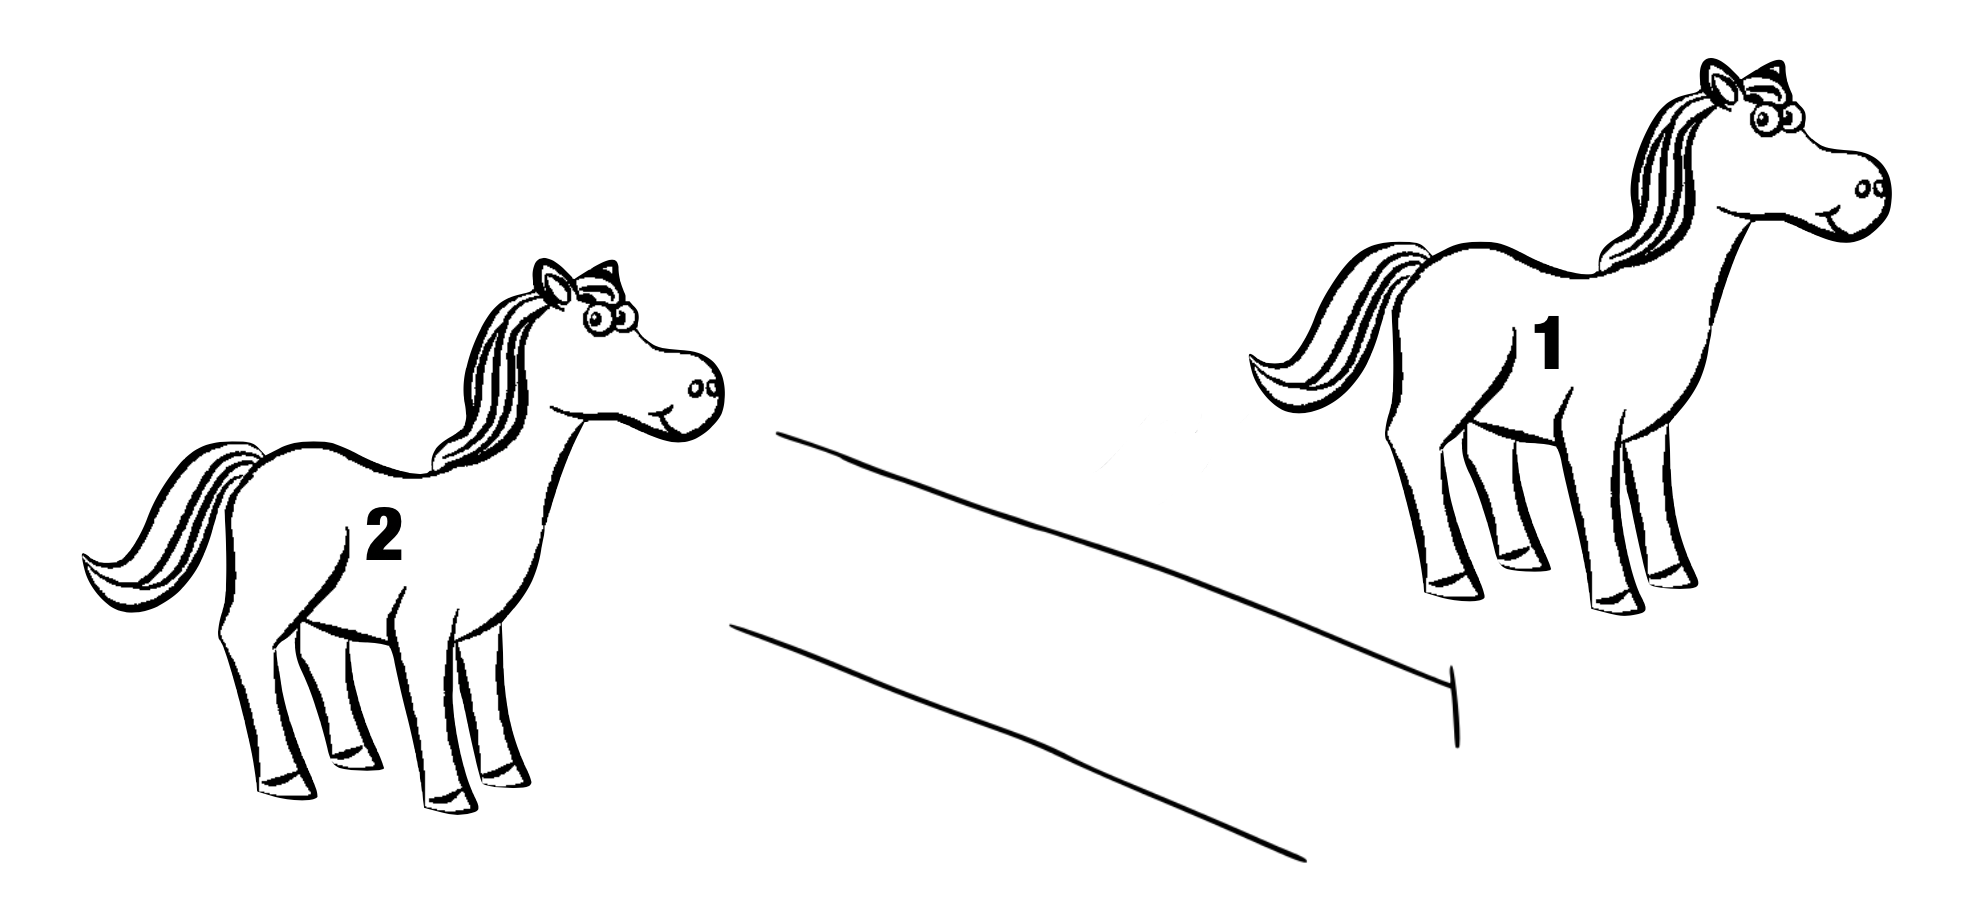
\includegraphics[width=4in]{not-all.png}
    \caption{Example not-all scenario in which horse 1 jumps over the fence but horse 2 does not. In this scenario, \ref{every-not-inverse} is true (not all of the horses jumped) but \ref{every-not-surface} is false (it is not the case that no horses jumped)}
    \label{not-all}
\end{figure}

In a not-all scenario of this sort, \lp{adults readily endorse statement \Last 
(90-100\% acceptance)
while five-year-old children typically do not (10-20\% acceptance) \citep{musolino1998,lidzmusolino2002,musolinolidz2006,musolino2006structure,viauetal2010,tieu2015}. }
% %that 
% adults can access both 
% %surface and inverse 
% interpretations,
% %of sentences like \Last. However, 
% five-year-old children have been reported to struggle with the inverse scope interpretation in \Last[b] \citep{musolino1998,lidzmusolino2002,musolinolidz2006,musolino2006structure,viauetal2010,tieu2015}. In more detail, when presented with a not-all scenario as in Figure \ref{not-all}, adults readily endorse \Last as a suitable description of the scene (90-100\% acceptance), whereas children typically do not endorse the sentence (10-20\% acceptance). 
\lp{Following the implicit linking hypothesis mentioned above for the truth-value judgment task, these child judgments have been interpreted to mean that children struggle to access the inverse interpretation of sentences like \Last the way that adults can.} 
%Taking these facts at face value, we might conclude that children's grammars are incapable or generating the inverse interpretation that would verify Figure \ref{not-all}; alternatively, we might conclude that children are incapable of accessing this interpretation given the available processing resources. 
\lp{The interesting question is {why children struggle}, and there are several possibilities that have been discussed in the literature cited above. 
%\lsp{probably need to cite the people who say this? Probably the child researchers above?}. 
Perhaps children are unable generate the inverse interpretation at all because their semantic knowledge is still developing (a grammatical factor). 
Perhaps children can generate the inverse interpretation, but not access it in the truth-value judgment task because of their developing processing abilities (a grammatical factor).
Perhaps children can generate and access the inverse interpretation, but choose not to endorse the test sentence for other---typically pragmatic---reasons (e.g., children don't believe the sentence is a reasonable thing to say, given the story scenario); this resistance to endorsement would be due to one or more pragmatic factors.
}

%However, these conclusions would be premature. 
\lp{Interestingly,} \lp{strategic} changes to the 
%truth-value-judgment-task 
\lp{truth-value judgment task}
setup lead to more adult-like behavior, such that children more readily endorse sentences like \ref{every-not} in a not-all scenario as in Figure \ref{not-all} \citep{viauetal2010}. 
%% but teasing apart these explanations is still hard
\lp{However, despite the carefully-designed manipulations of the experimenters, it often remains unclear which factors are responsible for children's differing behavior: grammatical factors, pragmatic factors, or both. This is where computational cognitive modeling can help us.}

\subsection{\lp{Computational cognitive modeling of the truth-value judgment task}}
%\lsp{Lisa start here: Slightly reorder this. 
%Start with how comp cog models can help, because they formally articulate theories of the underlying cognitive processes (here: ambiguity resolution in context, via the truth-value judgment task).
%Then go back to how they help in this scenario: they can explain whether the child-adult differences are due to grammatical, pragmatic, or both. 
%In particular, they can explain (i) how an adult does it, (ii) how a child does it, and so (iii) what has to change to go from being a child to being an adult. 
%When we understand these, we understand the truth-value judgment task better, which means we know better how to interpret the judgment data from it. We can also generate predictions for judgment data we expect to see with certain experimental setup manipulations. Then: specifically here, we use the RSA. 
%}

% Here, our hypotheses concerning the mapping between cognitive mechanisms and observable behavior in the truth-value judgment task are presented in the form of computational cognitive models. 
%Such models allow for (and enforce) the articulation of cognitive theories, identifying how different components of underlying knowledge interact to produce observable behavior \citep[e.g.,][]{pearlsprouse2015,pearl2017}.
\lp{Computational cognitive models implement cognitive theories concretely. In particular, a computational cognitive model articulates how different components of underlying knowledge interact to produce observable behavior \citep[e.g.,][]{pearlsprouse2013,goodmanfrank2016,pearlmis2016,pearl2017,pearletal2017,pearl2018chapter, pearlsprouse2018linking, scontrasetalproblang}.
Here, we use computational cognitive modeling to implement cognitive theories of ambiguity resolution in context, specifically how a participant (child or adult) would resolve a quantifier scope ambiguity like \Last in story contexts like Figure \ref{not-all}.
By articulating how different cognitive components interact---both grammatical and pragmatic components---a computational cognitive model can predict not only which factors contribute to the observed truth-value judgment endorsement behavior, but also how much each factor contributes.
Doing so allows us to transparently untangle the separate contributions of each factor.}

Applying a modeling approach to the question of truth-value judgments for scopally-ambiguous utterances, \lp{ we can identify which cognitive factors lead to adult-like judgments and how they do so. We can then see if these same factors can lead to child-like judgments, and, if so, how they do so. When we have potential explanations for both adult behavior and child behavior, we can then articulate a developmental theory: what needs to change for children to become adult-like.}
%When we understand these, we understand the truth-value judgment task better, which means we know better how to interpret the judgment data from it. 
 \lp{More generally, when we understand how the underlying cognitive factors can yield observable endorsement behavior in the truth-value judgment task, we better understand the truth-value judgment task itself, and how to interpret truth-value judgment results.}
% Understanding why 
% \lp{truth-value judgment experimental setup}
% changes have the effects that they do informs not only the differences between children and adults, but also the cognitive mechanisms that deliver observable behavior in the
% %truth-value judgment 
% \lp{truth-value judgment}
% task.
%In other words, understanding task behavior promises to inform our understanding of the task itself, thereby allowing for a cleaner mapping between our theories and the data that test them.

%We can also generate predictions for judgment data we expect to see with certain experimental setup manipulations. Then: specifically here, we use the RSA.
 An additional benefit of \lp{computational cognitive} models that 
 \lp{predict observable behavior (such as the endorsement behavior in a truth-value judgment task)}
 % explicitly aim to output behavior 
 is that model predictions can then be tested by further behavioral work. If we find that the modeling predictions match what humans do
 \lp{(e.g., truth-value judgment endorsement rates for other contexts and/or test sentences)}, we have strong support for the model-\lp{implemented} theory of how the underlying components interact. 



\subsection{\lp{The rest of this paper}}
This paper is structured as follows. We begin 
%in Section \ref{background}
with an overview of the empirical facts concerning children's ambiguity-resolution behavior in 
%truth-value judgment 
\lp{truth-value judgment}
tasks, together with the relevant task manipulations that make children more adult-like. 
%Section \ref{every-not-model} 
\lp{We then}
present our computational \lp{cognitive} model of utterance endorsement in the 
%truth-value judgment 
\lp{truth-value judgment}
task,
%\lsp{Maybe here's the place to mention the RSA, rather than the subsection above?}.
% Our model of utterance endorsement in the truth-value judgment task 
\lp{which}
is conceived within the Bayesian Rational Speech Act modeling framework (\citealp{goodmanfrank2016}; \citealp{scontrasetalproblang}). 
\lp{With this model}ing approach, we demonstrate how both child and adult \lp{truth-value judgment endorsement} behavior can be captured using a single model with different parameter settings.
In other words, we show how \lp{the same cognitive factors can interact in the same way to produce either child-like or adult-like behavior. The difference}s are quantitative in nature, such that different values for the same factor yield diverging behavior.
%is what the value of each factor is.
\lp{That is, our model predicts that adults and children} 
 are \lp{in fact} performing the same pragmatic calculus when evaluating ambiguous utterances in the 
\lp{truth-value judgment task.}
%, thereby offering insight into differences between children and adults. 

\lp{Given this finding, our model}
predicts that adults should be affected by the same sorts of task manipulations that have been found to modulate children's behavior.
We explore this prediction, 
%in Section \ref{two-not-model}, where we 
consider\lp{ing}
\lp{truth-value judgment data for}
a case of ambiguity that leaves adults looking like children.
\lp{We demonstrate how our model can be extended to capture this adult truth-value judgment task behavior, underscoring how the same underlying cognitive variables interacting in the model-specified way can account for a variety of truth-value judgment task data.}
\lp{More generally, our findings suggest that child and adult truth-value judgment behaviors are driven by the same underlying cognitive factors, but with different values for those factors. So, to become adults, children do not need to qualitatively change how they resolve scope ambiguity; this finding supports the continuity hypothesis}
%By extending our model to capture both child and adult behavior, we offer support for the hypothesis of continuity 
  in the development of scope-ambiguity resolution from childhood into adulthood. 
  \lp{We conclude by}
  %Section \ref{discussion} 
  synthesizing our findings and discussing their implications for our understanding of language development and 
  \lp{methods that can be fruitfully used to assess that development.}
  %linguistic meaning.



\section{
%Background
\lp{Children on the truth-value judgment task}
} \label{background}

% Children often deviate from adults in the truth-value judgment task when presented with sentences as in \ref{every-not}, repeated in \ref{every-not-repeat}.



% Adults charitably interpret the ambiguous utterance in a way that makes it a true statement, endorsing the utterance in a not-all scenario as in Figure \ref{not-all}. In contrast, five-year-old children
% stick with the surface interpretation in \ref{ex:surface}, which is false.

Children's behavior with scopally-ambiguous utterances in the 
%truth-value judgment 
\lp{truth-value judgment}
task has been shown to be sensitive to manipulations of the experimental context. In the basic task, children are presented with a background story about the agents---for example, horses engaging in some activities.  After this background story, children watch as the agents attempt to complete an action, such as jump over a fence. The critical not-all result state meant to prompt the inverse scope interpretation is illustrated in Figure \ref{not-all}, where \lp{horse 1 jumps over the fence and} horse 2 does not. In this scenario, the surface interpretation of the sentence in \ref{every-not}, repeated in \ref{every-not-repeat}, is false \lp{(again, because horse 1 did jump; therefore, none jumped is false)},  and the inverse scope interpretation is true \lp{(again, because horse 2 didn't jump; therefore not all jumped is true)}.  

\ex. \label{every-not-repeat}
Every horse didn't jump over the fence.
\a. \label{every-not-surface-repeat}
\textsc{Surface scope} ($\forall > \neg$):\\
None of the horses jumped over the fence.
\b. \label{every-not-inverse-repeat}
\textsc{Inverse scope} ($\neg > \forall$):\\
Not all of the horses jumped over the fence. 

A puppet then produces an utterance, such as the sentence in \ref{every-not-repeat}, and the child is asked to state if the puppet is right. That is, the child is asked  whether s/he would endorse the puppet's utterance as a true description of the scenario. Typically, children  refuse to endorse the puppet's utterance in inverse-verifying scenarios like in Figure \ref{not-all}, saying that the puppet is wrong; \lp{in contrast,} adults readily endorse the utterance \lp{in this context}. This behavior has been interpreted as children failing to access the inverse scope interpretation that would make the utterance true. 
\lp{That is, if children could access the inverse scope interpretation, they would recognize that \emph{not all of the horses jumped over the fence} is true in this scenario, and therefore they should endorse the scopally-ambiguous utterance in \ref{every-not-repeat}.} But given that children typically do not endorse the utterance in this scenario, children's behavior is interpreted as evidence that they must not access the inverse scope interpretation.

Previous accounts of children's scope-interpretation behavior have recognized that both processing and pragmatic factors may contribute to non-adult-like behavior. \cite{musolino1998,musolino2006structure} observed that the surface scope interpretation in \ref{every-not-surface-repeat} may be easier to process because the scope relationship at logical form (i.e., $\forall > \neg$) aligns with the  linear order of these elements in the utterance (i.e., \textit{Every} precedes \textit{n't}). In contrast, for the inverse scope interpretation in \ref{every-not-inverse-repeat}, this parallelism does not hold,  with the scope relationship (i.e., $\neg$ scopes over $\forall$) opposite the linear order of the elements in the utterance. Musolino hypothesized that this lack of parallelism would make the inverse scope interpretation more difficult to access. In line with this prediction, \cite{conroyetal2008} found that when adults are time-restricted, they favor the surface scope interpretation. We thus see a potential role for processing factors in children's inability to access the inverse scope. Perhaps children, with their still-developing processing abilities, are unable to allocate sufficient processing resources to reliably access the inverse scope interpretation.

In addition to this processing factor, \cite{gualmini2008question} noted that discourse properties, such as what children consider to be the question under discussion (QUD), may impact their scope-interpretation behavior.  Formal theories of pragmatics suggest that all discourse transpires with respect to some QUD, whether implicit or explicit; utterances in the discourse need to (at least partially) answer the QUD to be pragmatically felicitous \citep{roberts2012information}. Gualmini and colleagues \citep{hulsey2004question, gualmini2008question} suggest that children are very sensitive to this requirement. In particular, children may be able to access the inverse scope interpretation but nonetheless choose the surface scope interpretation because it better answers the perceived QUD in the contrived experimental setups. So, children's observed behavior would derive from a still-developing ability to manage the contextual information available and correctly infer the intended QUD.

Interestingly, various alterations to the %truth-value-judgment-task 
\lp{truth-value judgment task}
setup have yielded more adult-like behavior in children---namely, greater rates of endorsing the puppet's ambiguous utterance in not-all scenarios. \cite{musolinolidz2006} hypothesized that negation in an utterance might require certain felicity conditions to be met. In particular, negated utterances require a preceding affirmative context with which to contrast \citep{wason1965contexts}.  \citeauthor{musolinolidz2006} augmented the basic %truth-value judgment 
\lp{truth-value judgment}
task to include an additional contrast condition in which the puppet precedes its negative scopally-ambiguous utterance with a contrasting affirmative clause. This additional clause describes a previous successful story action (an ``early success''),  as in \textit{Every horse jumped over the log, but every horse didn't jump over the fence}. This early-success contrast manipulation increased children's willingness to accept the scopally-ambiguous utterance in the {not-all} scenario: children in the baseline condition endorsed the puppet's statement just 15\% of the time, while children in the early-success condition endorsed the puppet's statement 60\% of the time. \cite{viauetal2010} replicated this increase in utterance endorsement using only an early-success story context. That is, the higher utterance endorsement rate was maintained by an early-success story context alone; children did not need an explicit contrast clause in the test utterance 
\lp{(instead hearing only a scopally-ambiguous utterance like \textit{Every horse didn't jump over the fence}, just as in the original experiments by \citeauthor{musolinolidz2006})}.

Notably, the early-success affirmative-context manipulation  potentially changes several aspects of the experimental context.  First, observing early successes can shift participants' expectations about successful outcomes more generally in the experimental world. This shift then potentially increases the salience of a QUD targeting this success, such as \textit{did all the horses succeed?} (\texttt{all?}). Recognizing this QUD's potential significance, \cite{gualmini2004some} attempted to manipulate the experimental context so it favored the \texttt{all?}~QUD. With \texttt{all?}~as the salient QUD, children's endorsement of a scopally-ambiguous utterance that perfectly answered \texttt{all?}~in the critical not-all scenario increased to 90\%.  Even for a scopally-ambiguous utterance that does not fully answer the \texttt{all?} QUD, children's endorsement rate was at 50\% with the \texttt{all?} QUD---markedly higher than the 15\% baseline from the original study by \cite{musolinolidz2006}. This finding highlights that privileging the \texttt{all?} QUD increases children's utterance endorsement in these scenarios.
 
In addition to altering expectations about likely states of the world and QUDs, a third potential impact of the early-success affirmative-context manipulation involves scope access. By  altering the experimental world expectations and/or expectations about the QUD to increase access to the inverse scope, the inverse scope interpretation may also remain more accessible for later use.  \cite{viauetal2010} term this prolonged increase in accessibility ``structural priming''.  Children who are better able to access the inverse scope are then more likely to endorse the scopally-ambiguous utterance in subsequent {not-all} scenarios. \citeauthor{viauetal2010}~investigated structural priming explicitly by attempting to directly alter the accessibility of the inverse scope interpretation. In one modified 
%truth-value judgment 
\lp{truth-value judgment}
task, the authors attempted to prime the access of the inverse scope interpretation; in another modified task, they attempted to directly prime the inverse scope's logical structure (e.g., $\neg>\forall$).

The first structural priming manipulation was implemented via the now-familiar early-success affirmative-context manipulation. For the first three trials, the  prior experimental context indicated successful outcomes; the effect was that children endorsed the scopally-ambiguous utterance 50\% of the time. Crucially, the subsequent three trials removed the supportive affirmative-context manipulation, yet children continued to not only endorse the scopally-ambiguous utterance, but to endorse it more than they had before (80\% endorsement). \cite{viauetal2010} attribute this result to a priming effect of the inverse interpretation from the first three trials: having accessed the inverse structure in the early trials, children are more likely to access that same structure in later trials. However, the increase in utterance endorsement could be due to the privileging of multiple  factors that are products of the affirmative-context manipulation: (i) expectations about successful outcomes in the experimental world, (ii)  the salience of the \texttt{all?} QUD, or (iii)  the ease of access to the inverse scope interpretation. 

The second structural priming manipulation removed the affirmative-context story in the first three trials. In its place, children were asked whether they would endorse a scopally-unambiguous utterance (e.g., \textit{not every horse jumped over the fence}), whose interpretation had logical operators in the same configuration as the inverse scope interpretation of the scopally-ambiguous utterance (i.e., $\neg>\forall$). Children endorsed this utterance 80\% of the time. In the subsequent three trials, children were asked if they would endorse the scopally-ambiguous utterance in the same experimental scenario---and their endorsement rate remained at 80\%. \cite{viauetal2010} interpret this effect as priming of the relevant logical form: the inverse scope was easier to access in the scopally-ambiguous utterance because it was recently accessed in the unambiguous utterances. The authors argue that this priming effect proceeded in the absence of manipulations to the pragmatic context; yet, even here there may still be pragmatic factors at work. The unambiguous utterance accomplishes three things: (i) it provides an instance of the $\neg>\forall$ configuration, (ii) it provides information about successful outcomes, and (iii) it suggests the \texttt{all?}~QUD, answering it with \emph{no}. Thus, in this attempt to prime the inverse logical form, the authors may have also altered expectations about the pragmatic context of the experiment as it relates to successful outcomes and relevant QUDs.

These experimental studies highlight at least three core factors (two pragmatic, one \lp{grammatical} processing) that underlie children's utterance endorsement behavior in the 
%truth-value judgment 
\lp{truth-value judgment}
task: (i)  pragmatic: expectations about the experimental world (e.g., how likely successful outcomes are), (ii) pragmatic: expectations about the QUD (e.g., if it is relevant to establish whether all outcomes were successful), and (iii) \lp{grammatical} processing: the accessibility of the inverse scope (i.e., the ease by which the logical form is accessed). These experimental studies have also supported different theoretical proposals for the source of children's differences. The proposals split on whether they attribute the differences solely to an inability to manage contextual information (i.e., pragmatic factors; \citealp{gualmini2008rise}) or whether \lp{grammatical} processing deficits also significantly contribute (i.e., difficulty accessing inverse scope; \citealp{viauetal2010}). Importantly, it is not obvious from any of the existing experimental manipulations how to separate the independent contributions of these components. To capture and independently manipulate the contributions of each of the pragmatic and \lp{grammatical} processing factors, we formalize their role in the interpretation of scopally-ambiguous utterances, using tools from %probabilistic 
\lp{computational cognitive} modeling.


\section{
\lp{A computational cognitive model for \emph{every-not} utterances}
%\emph{Every-not} model
} \label{every-not-model}

We model  ambiguity resolution within the Bayesian Rational Speech Act (RSA) modeling framework \citep{goodmanfrank2016}, which views language understanding as a social reasoning process. A \textit{pragmatic listener} $L_1$ interprets an utterance by reasoning about a cooperative \textit{speaker} $S_1$ who is trying to inform a \textit{literal listener} $L_0$ about the world. Our model is a ``lifted-variable'' extension,
\lp{in which}
%wherein 
the ambiguous utterance's literal semantics is parameterized by interpretation-fixing variables (e.g., 
%the relative scope of the quantificational elements
\lp{whether the scope is surface or inverse}). Hearing an ambiguous utterance, a pragmatic listener reasons jointly about the true state of the world (e.g., how many horses jumped over the fence), the scope interpretation that the speaker had in mind (i.e., surface vs.~inverse), as well as the likely QUD that the utterance addresses (e.g., \texttt{how-many?} vs.~\texttt{all?}).  

To connect our model's predictions with the available %truth-value judgment 
\lp{truth-value judgment}
data, we follow recent suggestions in the literature 
\lp{for how to treat truth-value judgments.}
\lp{In particular, truth-value judgments are not viewed}
%for treating truth-value judgments not 
as pure language comprehension behavior, but rather as a form of language production (e.g., \citealp{degengoodman2014, jasbietal2019}).
%% say why not
% \lp{This is because the participant isn't hearing an utterance and comprehending what scenario that utterance could refer to (which would be typical language comprehension behavior).
A participant in the truth-value judgment task \lp{is shown a scenario and asked if a specific utterance can accurately describe that scenario. In this way, the truth-value judgment task seems to be asking if a speaker should describe the given scenario with the test sentence---that is, a type of production task.
}
\lp{If the participant judges the utterance as a reasonable description, the participant endorses the utterance in the truth-value judgment task. So, the participant has to effectively reason about her own potential production.}
%, or would it be better to say nothing at all? 
%In other words, 
\lp{Given this,}
we model participants' 
%truth-value judgment 
\lp{truth-value judgment}
behavior as the (relative) endorsement of  a \textit{pragmatic speaker} $S_2$ for an utterance about an observed situation; $S_2$ makes this decision by reasoning about the probability that $L_1$ (who is reasoning about $S_1$'s reasoning about $L_0$) would arrive at the correct world state after hearing the utterance. 


\subsection{Model specification}

We take world states $w\in W$ to correspond to the number of successful outcomes, for example, the horses that successfully jumped over the fence ($W=\{0,1,2\}$); the world success baserate $b_{suc}$ determines the probability that any individual will succeed. We assume a simple truth-functional semantics where an utterance $u$ denotes a mapping from world states to truth values ($Bool = \{\texttt{true},\texttt{false}\}$). We parameterize this truth function so that it depends on the scope interpretation $i \in I = \{\texttt{inverse}, \texttt{surface}\}$, \sem{\textit{u}}$^{i}$: $W\rightarrow$ \emph{Bool}. We consider two alternative utterances $u \in U$: the \texttt{null} utterance (i.e., saying nothing at all, and so choosing not to endorse the utterance) and the scopally-ambiguous utterance \texttt{amb} (e.g., \textit{``Every horse didn't jump over the fence''}); $U$ = \{\texttt{null}, \texttt{amb}\}. The utterance semantics appears in \ref{ex:utt-sem1}, where the interpretation parameterization only impacts the truth value for utterance \texttt{amb} (since only \texttt{amb} has multiple interpretations available). If \texttt{inverse} is active, \texttt{amb} receives a ``not-all'' reading and is true so long as not all outcomes were successful (i.e., $w\neq$2). If  \texttt{surface} is active, \texttt{amb} receives a ``none'' reading, which is true only in a world with zero successes \lp{(i.e., $w=0$)}.

\ex. \label{ex:utt-sem1} \emph{Utterance semantics} \sem{\textit{u}}$^{i}$:
\a. \sem{\texttt{null}}$^{i}$ = \texttt{true}
\b. \sem{\texttt{amb}}$^{i}$ = if $i$ = \texttt{inverse}, then  \sem{\texttt{inverse}}, else \sem{\texttt{surface}}\\[5pt]
 where: \sem{\texttt{inverse}} = $\lambda$w. w $\neq$ 2 \\
\phantom{where:} \sem{\texttt{surface}} = $\lambda$w. w = 0


We consider three QUDs $q \in Q$: 
(i) ``How many horses succeeded?" (\texttt{how-many?}), 
(ii) ``Did all of the horses succeed?" (\texttt{all?}), and 
(iii) ``Did none of the horses succeed?" (\texttt{none?}). 
The QUDs serve as projections from the inferred world state to the relevant dimension of meaning, $q: W \rightarrow X$ \citep*{kaoetal2014,kaoetal2014metaphor}. In practice, the QUDs establish partitions on the possible world states, as shown in \ref{ex:qud-sem1}: \texttt{how-many?}~is an identity function on world states, \texttt{all?}~returns \texttt{true} only if  both outcomes were successful, and \texttt{none?}~returns \texttt{true} only if none of the outcomes were successful.

\ex. \label{ex:qud-sem1} \emph{QUD semantics} \sem{\textit{q}}:
\a. \sem{\texttt{how-many?}} = \lam w. w
\b. \sem{\texttt{all?}} = \lam w. w = 2
\b. \sem{\texttt{none?}} = \lam w. w = 0


The literal listener $L_0$ hears some utterance $u$ 
\lp{(e.g., \textit{Every horse didn't jump over the fence})}
with intended interpretation $i$ 
\lp{(e.g., \texttt{inverse})}
and returns a uniform distribution over those world states $w$ \lp{that are} compatible with the literal semantics of $u$
\lp{(e.g., $w \in \{0,1\}$)}.
 The function $\delta_{[\![u]\!]^{i}(w)}$ maps the Boolean truth value to a probability, 1 or 0
\lp{(e.g., \texttt{true} maps to 1)}.

\begin{equation*}
P_{L_{0}} (w | u, i) \propto \ \delta_{[\![u]\!]^{i}(w)}
\end{equation*}
To capture the notion that communication proceeds relative to a specific QUD $q$, $L_0$ must infer not only the true world state $w$, but also the value of the QUD applied to that world state, $\sem{$q$}(w) = x \in X$. When $q$ is \texttt{how-many?}, $X$ ranges over $W$; otherwise, $X$ ranges over \emph{Bool}. In other words, when $q$ is \texttt{how-many?}, $L_0$ infers whether $x$ is 0, 1, or 2; when $q$ is \texttt{all?}, $L_0$ infers whether $x$ is \texttt{true} (i.e., $w \in \{2\}$) or \texttt{false} (i.e., $w \in \{0, 1\}$); when $q$ is \texttt{none?}, $L_0$ infers whether $x$ is \texttt{true} (i.e., $w \in \{0\}$) or \texttt{false} (i.e., $w \in \{1, 2\}$).

\begin{equation*}
P_{L_{0}} (x | u, i, q) \propto \ \sum_{w}\delta_{x=[\! [ q ]\! ](w)} \cdot P_{L_{0}} (w | u, i)
\end{equation*}

The speaker $S_1$ chooses an utterance $u$ in proportion to its utility. Utterance utility concerns the chance of successfully communicating $q$'s answer (i.e., the answer to the QUD) to $L_0$. Thus, $S_1$ chooses utterances by maximizing the probability that $L_0$ arrives at the intended $x$ from $u$. This selection is implemented via a softmax function ($exp$) and free temperature parameter $\alpha$, which controls how ``rational'' the speaker will be in utterance selection. As $\alpha$ increases, $S_1$ is more likely to maximize utility.\footnote{RSA models also factor in the cost of the utterance, such that $S_1$'s utility seeks to minimize utterance cost. We assume that our utterances are equally costly---neither response in the truth-value judgment task imposes a greater cost \lp{as the participant is saying either ``yes'' or ``no''}---so the cost term cancels out.} 
% \lp{The higher $\alpha$ is, the more committed the modeled speaker is to an extreme (e.g., a slight preference for one option over another becomes a strong preference for that option); conversely, with an $\alpha<0$, the modeled speaker will soften preferences (e.g., a strong preference for one option over another becomes a slight preference for that option).}

\begin{equation*}
P_{S_{1}} (u | w, i, q) \propto  \ exp (\alpha \cdot log(L_{0}(x | u, i, q)))\\
\end{equation*}

Utterance interpretation happens at the level of the pragmatic listener $L_1$, who interprets an utterance $u$ to jointly infer the world state $w$, the interpretation $i$, and the QUD $q$. We therefore model ambiguity resolution as pragmatic inference over an under-specified utterance semantics (i.e., the interpretation variable $i$; \citealp{scontrasgoodman2017}). To perform this inference, $L_1$ inverts the $S_1$ model by Bayes' rule, and so the joint probability of $w$, $i$, and $q$ is proportional to the  likelihood of $S_1$ producing utterance $u$ given world state $w$, interpretation $i$, and QUD $q$, as well as the priors on $w$, $i$, and $q$.

\begin{equation*}
 P_{L_{1}} (w, i, q | u) \propto  \ P_{S_{1}} (u | w, i, q) \cdot P(w) \cdot P(i) \cdot P(q)
\end{equation*}

To model the utterance endorsement implicit in 
%truth-value judgment 
\lp{truth-value judgment}
behavior, we need one more level of inference. The pragmatic speaker $S_2$ observes the true world state $w$  and selects $u$ by inverting the $L_1$ model, thus maximizing the probability that a pragmatic listener would arrive at $w$ from $u$ by summing over possible interpretations $i$ and QUDs $q$ that accompany world $w$. In other words, $S_2$ chooses $u$ to communicate $w$ by simulating how $L_1$ would resolve $i$ and $q$ for each of the possible utterances.
% \lp{For example, $S_2$ chooses \textit{Every horse didn't jump over the fence} to communicate $w=1$ where only horse 1 jumped (but not horse 2), summing over  \texttt{inverse} and \texttt{surface} in combination with QUDs \texttt{how-many}, \texttt{all?}, and \texttt{none?}.}

\begin{equation*}
P_{S_{2}} (u | w) \propto \ exp(log \sum_{i,q} P_{L_{1}} (w, i, q | u))
\end{equation*}

\subsection{Model predictions}

To generate model predictions, we must fix various model parameters. The $S_1$ speaker rationality parameter $\alpha > 0$ is set to $1$ (i.e., no scaling of $S_1$'s utility). The priors $P(w)$ and $P(q)$ correspond to expectations for the discourse context (i.e., likely world states or QUDs). In  the  default  case,  we  set  these  priors  so that the individual success baserate $b_{suc}$ is set to 0.5 (i.e., horses have a 50\% chance of success) and the relevant QUDs have equal probability (i.e., $P(\texttt{how-many?}) = P(\texttt{all?}) = P(\texttt{none?}) = \frac{1}{3}$). The interpretation prior $P(i)$ corresponds to how easy it is to access the inverse scope interpretation. In the default case, $P$(inverse) = $P$(surface) = 0.5.

To better understand children's utterance endorsement behavior with scopally-ambiguous utterances, we can independently manipulate the values of the priors on $W$, $Q$, and $I$, and observe their impact on utterance endorsement in not-all scenarios. That is, we can systematically manipulate the relevant priors to test how pragmatic 
\lp{factors ($W$ and $Q$)} and processing factors 
\lp{($I$)}
contribute to non-adult-like utterance endorsement behavior in the 
%truth-value judgment 
\lp{truth-value judgment}
task.


\begin{figure*}[t]
\centering
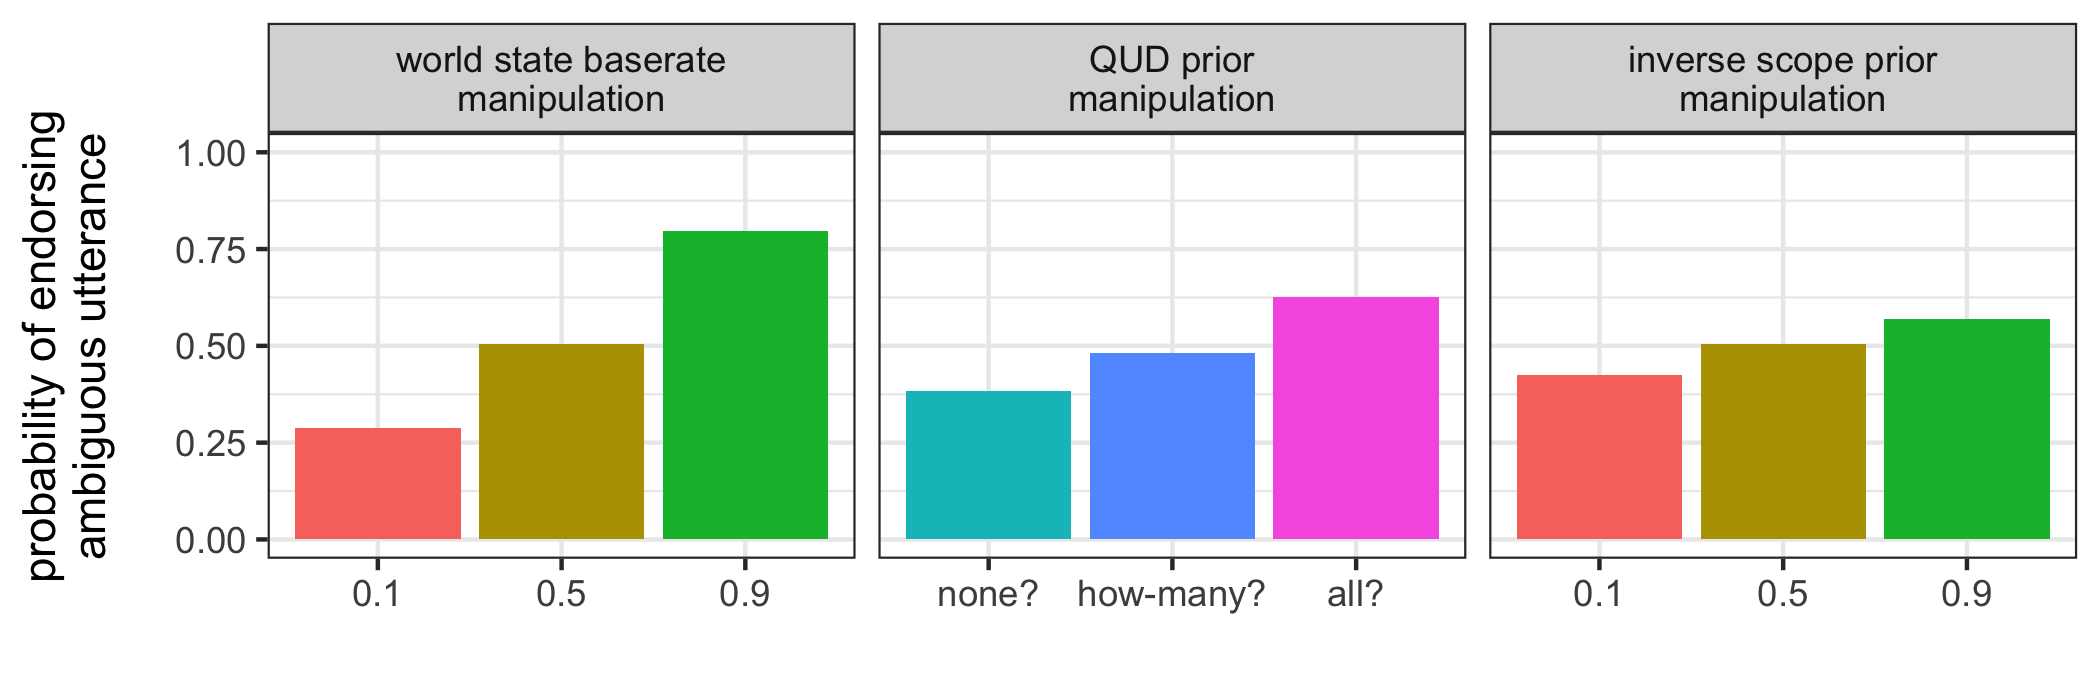
\includegraphics[height=1.55in]{every-not-plot.png}
%(natural priors: world = uniform.  scopes surface = .7 inverse = .3. QUDs = uniform)
%World state manipulation range (from 0 favored to 3 favored): .276 - .7524
%Scope Manipulation (from .1 favored inverse to .9 favored inverse): .3999 - .5716
%QUD manipulation (from none? favored to all? favored): .3171 - .6028
% \vspace{-15pt}
\caption{Model predictions for ambiguous utterance endorsement (e.g., \emph{Every horse didn't jump over the fence}) in a not-all scenario (e.g., one-out-of-two horses jump over the fence). Lower endorsement probability corresponds to less adult-like (i.e., more child-like) behavior. For the QUD factor, the favored parameter value receives most of the prior probability weight ($P(favored) = 0.9$). For the processing variable (scope), the prior corresponds to how strongly the inverse scope is favored}
\label{fig:every-not-plot}
\end{figure*}


To investigate the effect of manipulating the world state prior (Figure \ref{fig:every-not-plot}, \emph{left \lp{panel}}), we systematically alter the success baserate $b_{suc}$; in the horse context, $b_{suc}$ controls beliefs about how likely
horses are to succeed at jumping. Holding the QUD and scope priors at their default values, we see a marked increase in endorsement of the ambiguous utterance in the not-all scenario as beliefs about horse success increase. Utterance endorsement is at its lowest (0.29) when prior knowledge suggests that horses are particularly unlikely to succeed at jumping (i.e., that $b_{suc}$ is $0.1$); utterance endorsement is at its highest (0.80) when we believe horses are very likely to succeed (i.e., that $b_{suc}$ is $0.9$).

Just as with the world state prior, we can systematically manipulate the QUD prior (Figure \ref{fig:every-not-plot}, \emph{center \lp{panel}}).  Favored QUDs receive a prior probability of $0.9$; other QUDs receive a prior probability of $0.1/2=0.05$. Holding the other priors at their default values, we see an increase in utterance endorsement from the \texttt{none?} (0.38) to \texttt{how-many?} (0.48) to \texttt{all?} (0.63) QUD. %The model predicts the most adult-like behavior when the QUD concerns whether all the horses succeeded. 
\lp{So, utterance endorsement is at its lowest when we believe the QUD is about whether none of the horses jumped; utterance endorsement is at is highest when we believe the QUD is about whether all of the horses jumped.}

Finally, for the binary scope prior (Figure \ref{fig:every-not-plot}, \emph{right \lp{panel}}), we systematically manipulate the prior probability of \texttt{inverse} scope from $0.1$ to $0.9$. Holding the other priors at their default values, we see a monotonic increase in utterance endorsement as the probability of \texttt{inverse} increases. The model predicts an endorsement probability of 0.57 when the prior probability of \texttt{inverse} is at its highest ($0.9$)---at its lowest (0.1), endorsement drops to 0.42.
\lp{So, the more accessible the inverse interpretation, the more utterance endorsement increases---though notably, the change is less than the endorsement rate changes that occur by altering the pragmatic factors.}

To summarize, the world state and QUD priors have a more dramatic impact on utterance endorsement than the scope prior.  There are two main reasons for these predictions. First, for the world state prior, when expectations favor success, the ambiguous utterance is maximally informative regardless of the scope interpretation it receives: \texttt{amb} communicates to a listener that prior  expectations do not hold (i.e., \textit{None/Not all of the horses succeeded} goes against the expectation that all three horses would succeed, \lp{which is what high $b_{suc}$ entails}). So, \texttt{amb} is particularly useful for communicating about the \emph{a priori} unlikely not-all world states that appear in the experimental scenarios. Second, for the QUD manipulation, when \texttt{all?} is favored, either interpretation of \texttt{amb} fully resolves the QUD: whenever \texttt{amb} is true (i.e., whether none or not all of the horses succeeded), it is not the case that all of the horses succeeded. A pragmatic speaker recognizes the utility of \texttt{amb} as an answer to \texttt{all?} in a not-all world state, irrespective of the intended scope interpretation.
\lp{More generally, both pragmatic factors highlight that either scope interpretation will suffice if the right pragmatic context is present (a high $b_{suc}$ or the \texttt{all?} QUD).}
Thus, \lp{the model predicts that the processing factor (i.e., the inverse scope prior) should matter very little if both pragmatic factors are set so that either scope interpretation is informative. We demonstrate that this prediction is indeed true in Figure \ref{fig:interaction}.}


\begin{figure}[ht]
\centering
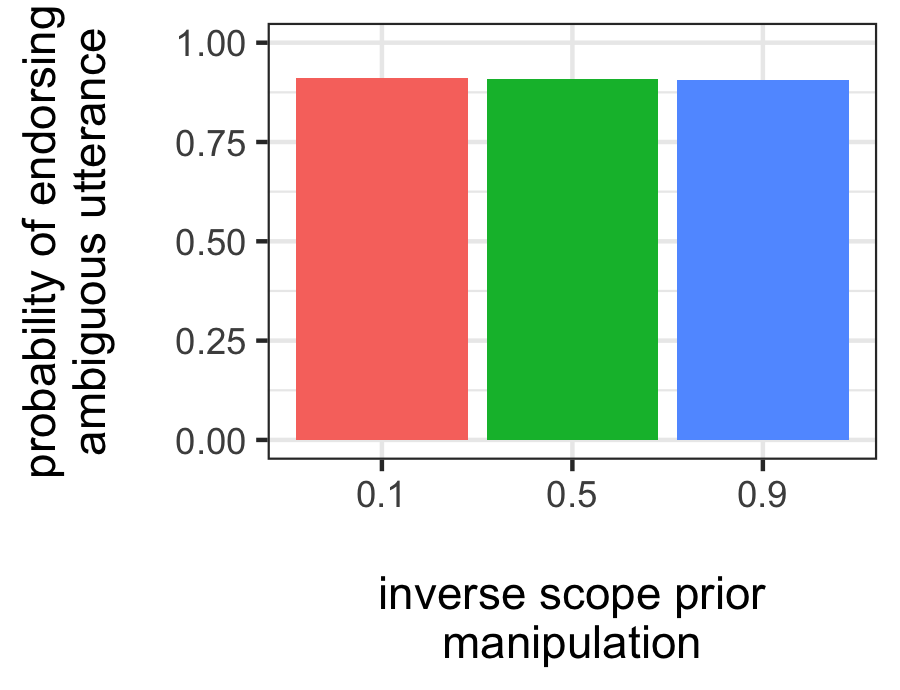
\includegraphics[height=1.55in]{every-not-pragmatic-plot.png}
% \vspace{-5pt}
\caption{Model predictions for ambiguous utterance endorsement when total-success world states are favored ($b_{suc}=0.9$) and the optimal QUD is favored ($P(\texttt{all?}) = 0.9$)}
\label{fig:interaction}
\end{figure}


%So far, we have considered independent manipulations to the factors of interest. 
\lp{In particular,} Figure \ref{fig:interaction} shows the interaction of all three factors for utterance endorsement when $b_{suc}=0.9$ and \texttt{all?}~are favored. We see the combined effects of the world state and QUD priors; together, they lead to near-total endorsement of the ambiguous utterance. %\lsp{(0.88?)}. 
We also see more clearly the relatively small contribution of the scope prior, where changing the prior probability of \texttt{inverse} from $0.1$ to $0.9$ leads to just a 0.002 change in endorsement probability.  Thus, we see how the priors on the pragmatic  factors overwhelm the processing factor of scope access. When the optimal QUD and world state are favored, even when \texttt{inverse} is highly inaccessible (i.e., $P(\texttt{inverse}) = 0.1$), we still predict high utterance endorsement (0.91).
\lp{That is, even if the inverse scope is very inaccessible, the model predicts high rates of endorsement for the truth-value judgment task when a supportive pragmatic context is present.}

\subsection{Discussion}

Our results suggest that when it comes to understanding non-adult-like behavior in the 
\lp{truth-value judgment}
%truth-value judgment 
task, there is a stronger role for the pragmatics of context management (as realized in priors on world state and QUD) than for grammatical processing (as realized in the prior on scope interpretations), although there may be a role for both. So, the observed failure of children to endorse scopally-ambiguous utterances in not-all scenarios likely stems more from children's beliefs about the world of the experiment (e.g., whether horses are \emph{a priori} likely to succeed) and about the topic of conversation (e.g., whether the conversational goal is to determine if all the horses succeeded) than an inability to grammatically derive or access the inverse scope interpretation. Indeed, our model predicts the highest rates of utterance endorsement when 
resolving the scope ambiguity is irrelevant for communicating successfully about the not-all world. In other words, the model predicts high endorsement whenever
\lp{the pragmatic context is supportive---}either because expectations favor total success or 
the QUD asks if \texttt{all?}~of the horses succeeded---\lp{irrespective of how difficult it is to access the inverse scope.}
%
\lp{This} prediction arises because
%In either case, 
both scope interpretations serve to inform a listener, either that the \emph{a priori} likely $w=2$ does not hold, or that the answer to the \texttt{all?}~QUD is \emph{no}. 
\lp{So, the non-adult truth-value judgment task behavior we see in children is predicted to stem from an inability to manage the pragmatic context; to become more adult-like in these scenarios, children must learn to adapt to less supportive pragmatic contexts.}

In the following section, we test the generalizability of our findings by exploring a case of ambiguity where adults start behaving like children.
If adults and children are using the same mechanism to resolve scope ambiguity in context \lp{(as implemented in our RSA model)}, we should find that similar contextual pressures affect endorsement behavior in both groups.
\lp{In particular, less supportive pragmatic contexts in these scenarios---due to the priors on world states or QUDs---should lead to lower endorsement rates} also in adults.



\section{\emph{Two-not}} \label{two-not-model}

% \subsection{\lp{Empirical truth-value judgment data}}
Over the course of three 
%truth-value judgment 
\lp{truth-value judgment}
tasks, \citet{musolinolidz2003} demonstrated that adults are sensitive to some of the same experimentally-manipulated factors as children when it comes to endorsing scopally-ambiguous utterances. Rather than looking at \emph{every-not} sentences, \citeauthor{musolinolidz2003} investigated sentences with negation and cardinal numerals \lp{like \textit{two}}, as in \ref{two-not}. As with \emph{every-not}, these \emph{two-not} sentences admit two interpretations, corresponding to the relative scope of the logical operators introduced by the numeral and negation.
% \lp{In particular, \texttt{surface} scope ($\exists > \neg$) is interpreted as there being two horses, each of which didn't jump over the fence; 
% \texttt{inverse} scope ($\neg > \exists$) is interpreted as it not being true that there are two horses who jumped over the fence.
% }
%Like us, \citeauthor{musolinolidz2003} were interested in developmental continuity: are child and adult ambiguity resolution behavior in context qualitatively similar? To investigate this, they conducted three truth-value judgmentTs. 

\newpage

\ex. \label{two-not}
Two horses didn't jump over the fence.
\a. \textsc{Surface scope} ($\exists > \neg$):\\
There are two horses that didn't jump over the fence.
\b. \textsc{Inverse scope} ($\neg > \exists$):\\
It's not the case that there are two horses that jumped over the fence.

\lp{One scenario that distinguishes between these interpretations is shown in Figure \ref{2-of-4}, where there are four horses total and two (horses 1 and 2) jumped over the fence while another two (horses 3 and 4) did not.
Here, the {surface} interpretation is true: there are in fact two horses, horses 3 and 4, that did not jump over the fence.
In contrast, the {inverse} interpretation is false: there are two horses that jumped over the fence (horses 1 and 2).}

\begin{figure}
    \centering
    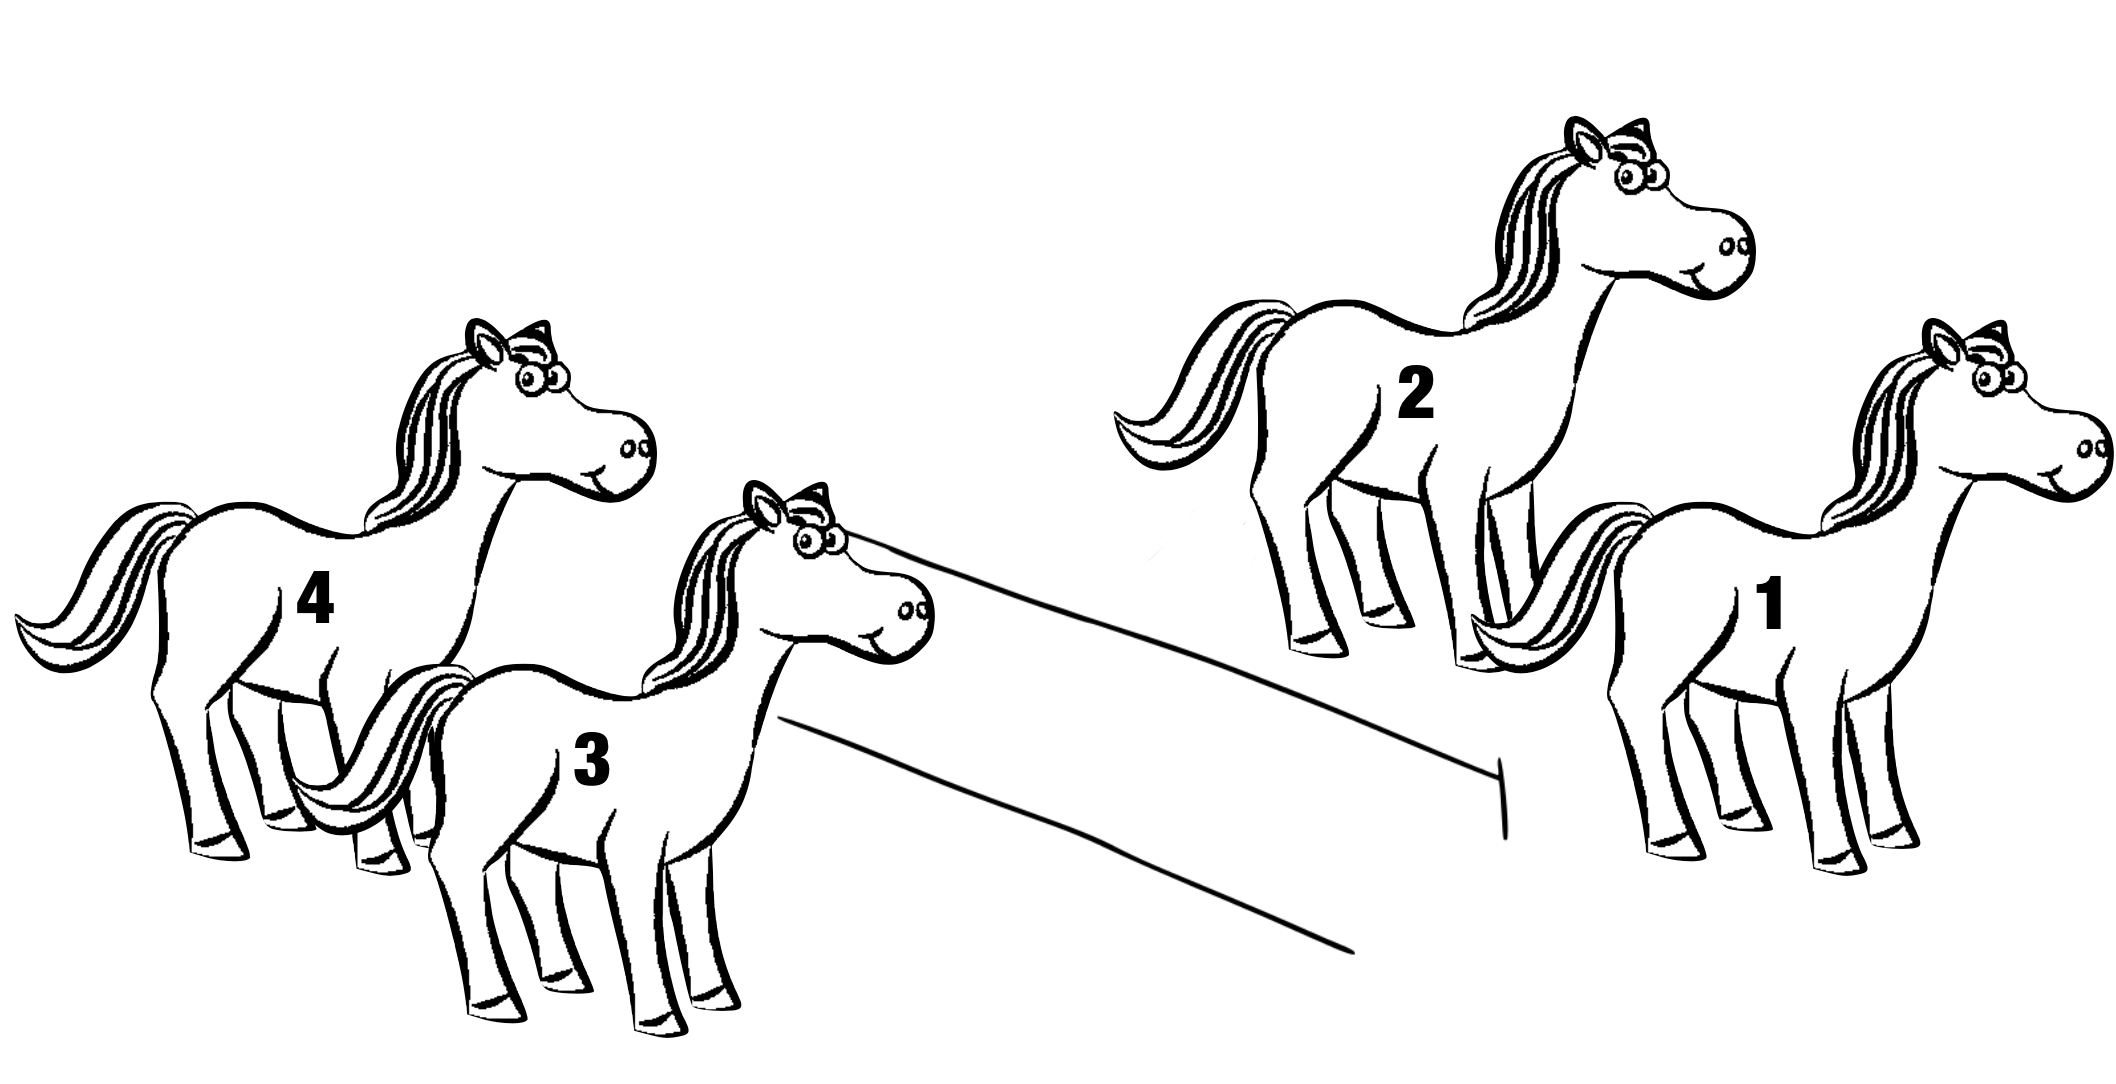
\includegraphics[width=4.5in]{2-of-4.png}
    \caption{Example 2-of-4 scenario in which horses 1 and 2 jump over the fence but horses 3 and 4 do not. In this scenario, only the \texttt{surface} interpretation of the \emph{two-not} sentence is true}
    \label{2-of-4}
\end{figure}


In the first task \lp{of \cite{musolinolidz2003}}, adults heard \emph{two-not} sentences in a context where both interpretations were true. 
\lp{For example, the scenario might} have one out of three horses jumping over a fence; 
\lp{the {surface} interpretation is true because there are two horses who did not jump; 
the {inverse} interpretation is also true because it is not the case that there are two horses who did jump}. 
After deciding whether to endorse the utterance, participants then justified their response so that their scope interpretation could be inferred. For example, if their explanation referred to the two horses that did not jump, then it was assumed that participants accessed the {surface} interpretation (there are two horses that didn't jump).
%\lsp{Can we check if this is right? Based on my walkthrough above, it seems like referring to the one horse jumping is about the inverse interpretation.}. 
However, if the explanation referred to only one horse jumping, then it was assumed that participants accessed the {inverse} interpretation (only one horse jumped, so it's not the case that two did).
% \lsp{Similar question---it seems like this would refer to the surface scope, based on the walkthrough above?}. 
\citeauthor{musolinolidz2003} found that all participants endorsed the utterance, and the  explanations provided indicated a strong surface scope bias (75\% {surface}, 7.5\% {inverse}, 17.5\% unclear from explanation). The authors interpreted this finding as evidence that adults prefer the {surface} interpretation of \emph{two-not} utterances when both interpretations are true in context. 
%It might then be the case that children's non-endorsement behavior for \emph{every-not} utterances, if due to a preference for the \textsc{surface} scope interpretation, is driven by a stronger version of this same preference.

In the second task, adults heard a \emph{two-not} sentence in two different contexts. The first context included two actors (e.g., horses), with one actor successfully completing the action (as in Figure \ref{not-all}; e.g., horse 1 jumped while horse 2 didn't). In this \textsc{1-of-2} context, the {surface} interpretation is false (only one horse didn't jump, so it is false that two horses didn't jump), but the {inverse} interpretation is true (only one horse did jump, so it is indeed not the case that two horses jumped). Adults exhibited low endorsement (27.5\%) for these \textsc{1-of-2} contexts. 

In the second context, there were four actors. For example, four horses attempted to jump over a fence; two jumped %\lp{(horses 1 and 2))} 
and two did not, %\lp{(horses 3 and 4)}, 
as in Figure \ref{2-of-4}.  In this \textsc{2-of-4} context, the {surface} interpretation of the scopally-ambiguous \emph{two-not} utterance is true: there are two horses that did not jump \lp{(horses 3 and 4 in Figure \ref{2-of-4})}. However, the {inverse} interpretation is false because there are two horses that did jump \lp{(horses 1 and 2)}. In these contexts, adults had an endorsement rate of 100\%. 



\citeauthor{musolinolidz2003} interpreted this asymmetry in endorsement rates between the two types of contexts, \textsc{1-of-2} vs.~\textsc{2-of-4}, as a strong {surface} scope preference in adults. According to this explanation,  non-endorsement occurs in the \textsc{1-of-2} context because only the {inverse} scope is true; in contrast, endorsement occurs in the \textsc{2-of-4} context because the {surface} scope is true. That is, both patterns arise because adults favor the {surface} interpretation. While we find this account compelling, we note that there are other differences between the two contexts that might lead to the observed asymmetry. For example, it could be that the seemingly benign change from two to four total actors affects the pragmatic context. Another variable is the potential ambiguity present in the numeral semantics, which only becomes relevant in the \textsc{2-of-4} context---we return to this ambiguity in the following subsection. In either case, exploring the effects of these factors in a formal model of 
%truth-value judgment 
\lp{truth-value judgment}
behavior \lp{like the one we implemented} above can clarify the process underlying utterance disambiguation. Before presenting such a model, we \lp{review one additional experiment}
%have one last experiment to review.
\lp{that investigates the impact of different experimental context manipulations on adult judgments.}
\lp{In particular, }
%Turning to the question of continuity in the development of ambiguity resolution behavior,
\citeauthor{musolinolidz2003} set out to determine whether adults are affected by the same factors as children when it comes to increasing utterance endorsement for scopally-ambiguous utterances. 

In their third task, the \citeauthor{musolinolidz2003} tested adults in  \textsc{1-of-2} contexts using an early-success manipulation familiar from the child 
\lp{truth-value judgment}
experiments reviewed above. With an early-success manipulation, adults saw a positive contrasting clause describing successful outcomes before the utterance of interest, as in \ref{two-not-early-success}.

\ex. \label{two-not-early-success} \textbf{{Two horses jumped over the rock, but}} \\
{two horses didn't jump over the fence.}

Adults responded just as the children did to the early-success contexts, shifting to strong endorsement (92.5\%; cf.~27.5\% endorsement without the explicit contrast).  However, as \citeauthor{musolinolidz2003} note, it is not obvious \emph{why} the adult endorsement rate increases when the early-success contrast is present. 

Here is where our model of utterance endorsement might be able to help: just as we did with \emph{every-not} utterances, we can model utterance endorsement for \emph{two-not} utterances in an attempt to formally explicate the contribution of context to the observed endorsement behavior. In the process, we can also test the hypothesis of continuity in the development of scope ambiguity resolution: if the same model architecture can capture both child and adult behavior, we have strong support for the hypothesis that children and adults are employing the same disambiguation mechanism.


\subsection{Model specification} \label{two-model-specification}

Our \emph{two-not} model is a direct extension of the \emph{every-not} model presented above. As before, we take world states $w\in W$ to correspond to the number of successful outcomes; the world success baserate $b_{suc}$ determines the probability that an individual will succeed. We continue to assume a simple truth-functional semantics where an utterance $u$ denotes a mapping from world states to truth values. As before, we parameterize this truth function so that it depends on the scope interpretation $i \in I = \{\texttt{inverse}, \texttt{surface}\}$, \sem{\textit{u}}$^{i}$: $W\rightarrow$ $Bool$. We consider two alternative utterances $u \in U$: the \texttt{null} utterance (i.e., saying nothing at all, \lp{which we take as equivalent to} choosing \emph{not} to endorse the utterance) and the scopally-ambiguous \emph{every-not} utterance \texttt{amb} (e.g., \textit{Two horses didn't jump over the fence}).  

To fix the utterance semantics, we must consider potential ambiguity introduced by the numeral in cases where the number of relevant individuals $n$ exceeds the numeral's value. For example, consider the positive utterance \textit{Two horses jumped over the fence.} If we assign an {exact} ($=$) semantics to the utterance, it will be true only when two horses succeeded. If we assign an {at-least} ($\geq$) semantics, the sentence will be true when two or more horses succeeded. In worlds with only two horses, the exact vs.~at-least distinction makes no difference: the sentence will be true in the world where both horses succeed, and false in all other worlds. However, in a world with four horses, the numeral semantics will define different truth-functional mappings. With the exact semantics, the sentence is true in any world where two horses---but not more---succeed. With the at-least semantics, the sentence is true in a larger set of worlds,  where two or more horses succeed. 

To evaluate the potential contribution of utterance semantics to the \textsc{1-of-2} vs.~\textsc{2-of-4} asymmetry, we consider two different sets of utterance alternatives, one with \texttt{amb$_{=}$} and another with \texttt{amb$_{\geq}$}. So, $U_{=}$ = \{\texttt{null}, \texttt{amb$_{=}$}\} and $U_{\geq}$ = \{\texttt{null}, \texttt{amb$_{\geq}$}\}. The utterance semantics in \ref{ex:utt-sem} shows that scope parameterization $i$ only impacts the truth conditions for \texttt{amb} utterances.
% \lp{
In our horse-jumping scenario, the
\texttt{inverse$_=$} interpretation returns \texttt{true} just in case the number of horses that jumped is not equal to two; similarly, 
% means it's not true that there are exactly two horses who jumped over the fence ($w \neq 2$);
\texttt{surface$_=$} returns \texttt{true} just in case the number of horses that jumped is equal to two.
% means there are exactly two horses who didn't jump over the fence (so when we have four horses, that means there are exactly two who did, $w=2$);
For the at-least interpretations, \texttt{inverse$_\geq$} returns \texttt{true} just in case the number of horses that jumped is less than two; 
% means it's not true that there are at least two horses who jumped over the fence (so when we have four horses, then zero or one jumped $\rightarrow$ less than two total jumped, $w<2$);
\texttt{surface$_\geq$} returns \texttt{true} just in case the number of horses that jumped is less than three.
% means there are at least two horses who didn't jump over the fence (so when we have four horses, then two, three, or four didn't jump $\rightarrow$ two, one, or zero did jump $\rightarrow$ less than three total jumped, $w<3$).
% }

\ex. \label{ex:utt-sem} \emph{Utterance semantics} \sem{\textit{u}}$^{i}$:
\a. \sem{\texttt{null}}$^{i}$ = \texttt{true}
\b. \sem{\texttt{amb$_{=/\geq}$}}$^{i}$ = \ \ \ \ if $i$ = \texttt{inverse} then \sem{\texttt{inverse$_{=/\geq}$}}\\
\phantom{\sem{\texttt{amb$_{=/\geq}$}}$^{i}$ = \ \ \ \ }else \sem{\texttt{surface$_{=/\geq}$}}\\
 where:\\
\sem{\texttt{inverse$_{=}$}} = $\lambda$w. w $\neq$ 2\\
\sem{\texttt{surface$_{=}$}} = $\lambda$w. w = 2\\
\sem{\texttt{inverse$_{\geq}$}} = $\lambda$w. w $<$ 2 \\
\sem{\texttt{surface$_{\geq}$}} = $\lambda$w. w $<$ 3



We consider five potential QUDs $q \in Q$, three from the \emph{every-not} model:
(i) ``How many horses succeeded?" (\texttt{how-many?}), 
(ii) ``Did all of the horses succeed?" (\texttt{all?}), and 
(iii) ``Did none of the horses succeed?" (\texttt{none?}). We also consider two additional QUDs specific to the \emph{two-not} utterance:  (iv) ``Did exactly two horses succeed?'' (\texttt{two$_=$?}), and
(v) ``Did at least two horses succeed?'' (\texttt{two$_\geq$?}).

\ex. \label{ex:qud-sem} \emph{QUD semantics} \sem{\textit{q}}:
\a. \sem{\texttt{what-happened?}} = \lam w. w
\b. \sem{\texttt{all?}} = \lam w. w = \texttt{max}(W)
\b. \sem{\texttt{none?}} = \lam w. w = 0
\b. \sem{\texttt{two$_=$?}} = \lam w. w = 2
\b. \sem{\texttt{two$_\geq$?}} = \lam w. w $\geq$ 2


\subsection{Model predictions}

To generate model predictions for adult sensitivity to the pragmatic contrast manipulation and the  \textsc{1-of-2} vs.~\textsc{2-of-4} asymmetry, we fix various model parameters. For \textsc{1-of-2} data, we set the number of individuals to 2 (i.e., \texttt{max}(W) = 2); for \textsc{2-of-4} data, we set the number of individuals to 4 (\texttt{max}(W) = 4). The $S_1$ speaker rationality parameter $\alpha > 0$ is set to $1$. As before, the priors $P(w)$ and $P(q)$ correspond to expectations for the discourse context. In the default case, we set the individual success baserate $b_{suc}$ to 0.5 and we set $P(q)$ so that the relevant QUDs have equal prior probability. The interpretation prior $P(i)$ corresponds to how easy it is to access the \texttt{inverse} scope interpretation. In the default case, P(\texttt{inverse}) = P(\texttt{surface}) = 0.5. \lp{As with the \textit{every-not} model},  we can independently manipulate the values of the priors on $W$, $Q$, and $I$, and observe their impact on utterance endorsement
\lp{in order} to better understand utterance endorsement behavior with scopally-ambiguous utterances.

Recall the empirical phenomena we are trying to capture: (i) the dramatic increase in endorsement rates in the \textsc{1-of-2} context when an explicit contrast is present, and (ii) the stark asymmetry in utterance endorsement rates between \textsc{1-of-2} and \textsc{2-of-4} contexts. We report results for each phenomenon in turn.

\subsubsection{The explicit contrast effect for \textsc{1-of-2}}

% \begin{figure*}[ht]
% \centering
% 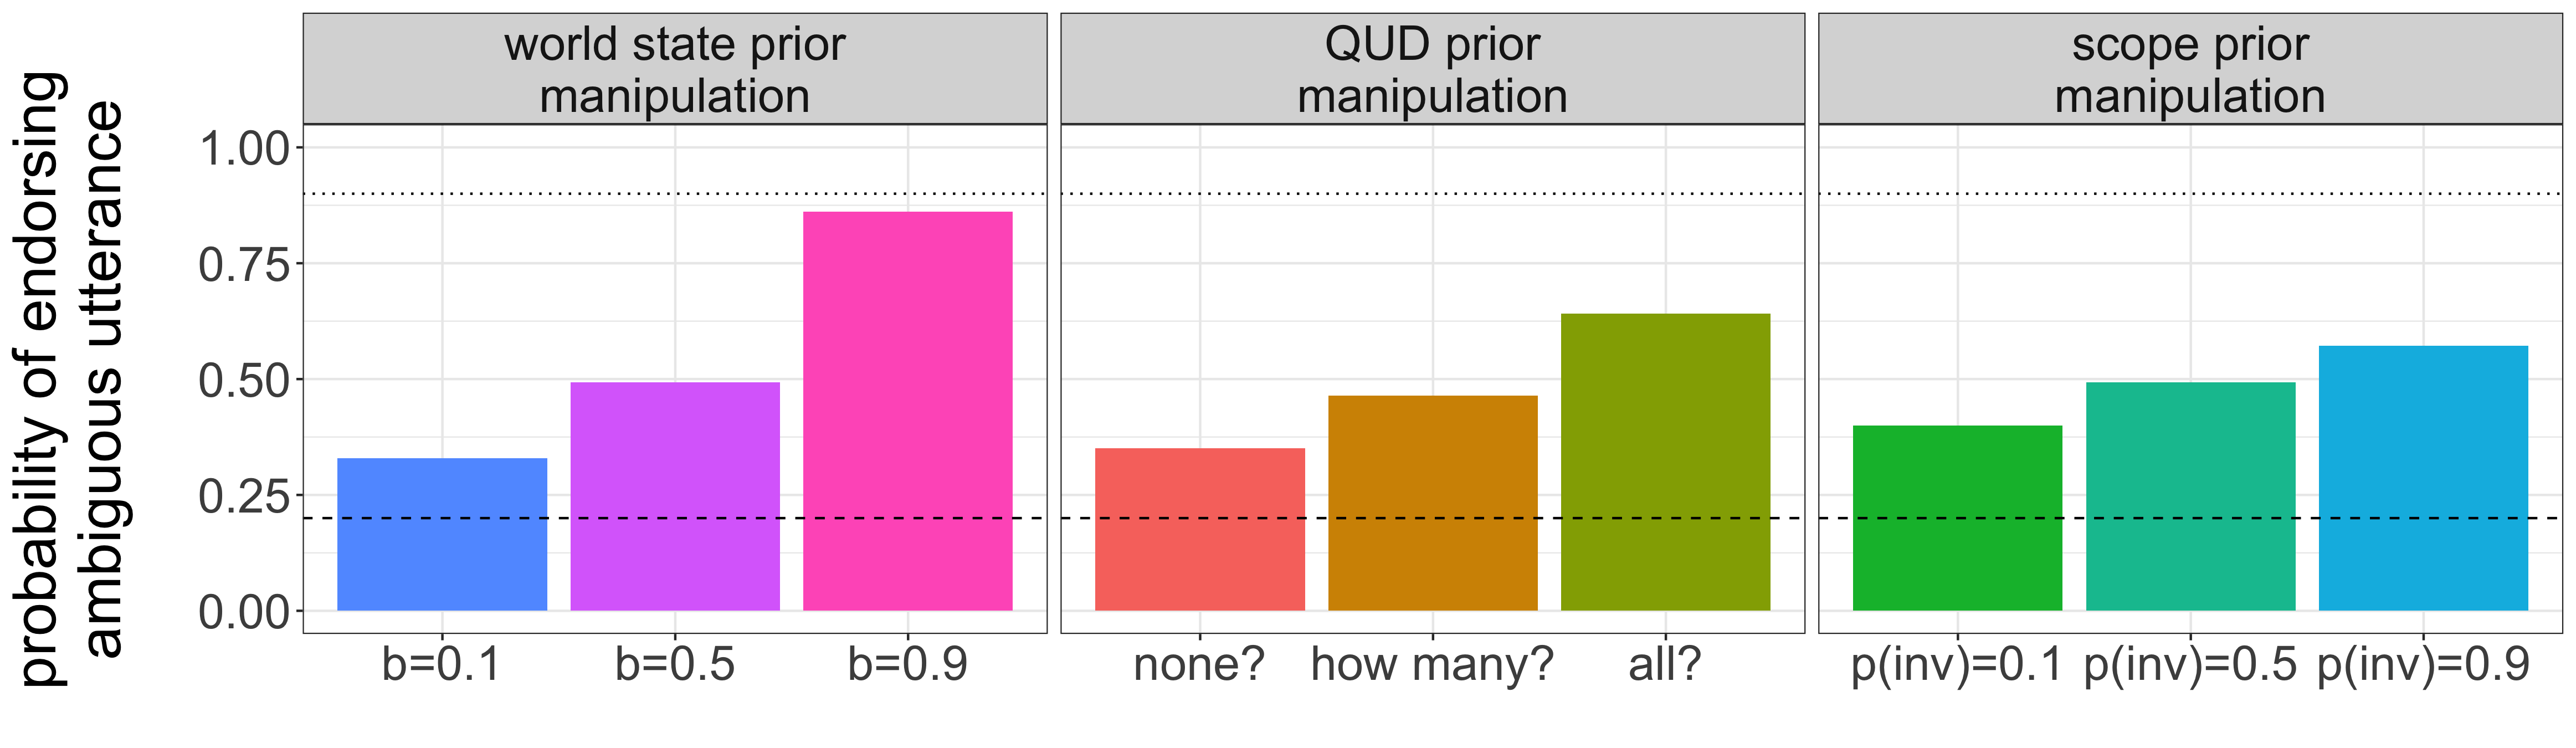
\includegraphics[width = .9\textwidth]{plots/CMCL-figure1.png}
% \vspace{-20pt}
% \caption{Model predictions for ambiguous \textit{two-not} utterance endorsement (e.g., \emph{Two frogs didn't jump over the rock}) in a \textsc{1-of-2} context. Dotted lines represent experimentally-observed endorsement behavior in the absence (lower) and presence (upper) of an explicit contrast.}
% \label{fig:independent}
% \vspace{-10pt}
% \end{figure*}

%As with the \emph{every-not} model, 
We can attempt to capture the increase in ambiguous utterance endorsement rates by systematically manipulating the pragmatic and processing factors, as implemented in the relevant priors. In a \textsc{1-of-2} context, the \emph{two-not} model predictions are identical to the predictions of the \emph{every-not} model in Figure \ref{fig:every-not-plot} above---the models align because the ambiguous \emph{two-not} and \emph{every-not} utterances, for both scope interpretations, wind up true of exactly the same world states when $W = \{0, 1, 2\}$. 
% some handholding
% \lp{
That is, the \texttt{surface} interpretation for the \textit{every-not} utterance 
% \textit{Every horse didn't jump over the fence} (\textit{$\forall > \neg$}) 
holds that all (i.e., two) horses failed to jump over the fence ($w=0$); 
the \texttt{surface} interpretation for the \textit{two-not} utterance 
%\textit{Two horses didn't jump over the fence} ($\exists > \neg$) 
is the same: two (i.e., all) horses failed to jump ($w=0$).
The situation is similar for the \texttt{inverse} interpretation: \emph{every-not} is true when not all of the horses jumped over the fence ($w = 0, 1$), and \emph{two-not} is true when the number of horses that jumped is not two ($w = 0,1$)
% \lp{For the \texttt{inverse interpretation} of \textit{every-not} ($\neg > \forall$), this means it's not the case that all (two) horses jumped over the fence ;
% for the \texttt{inverse} interpretation of \textit{two-not} ($\neg > \exists$), this means it's not the case that there are two horses that jumped over the fence ($w = 0,1$).
% }


By replicating the results of our manipulations for the \emph{every-not} model, each prior manipulation for the \emph{two-not} model qualitatively captures the response pattern from \cite{musolinolidz2003}. 
% let's remind them
%\lp{In particular,  the pragmatic factor priors (i.e., the world prior and the QUD prior) have a much stronger impact on the endorsement rate than  the grammatical processing prior (i.e., the inverse scope interpretation prior).}
\lp{In particular}, as before, the pragmatic factors controlling world and QUD beliefs have a much more pronounced effect than the processing factor controlling scope access; 
the model's world prior baserate manipulation comes closest to capturing the experimentally-observed effect of explicit contrast manipulation (i.e., 27.5\% base endorsement vs. 92.5\% endorsement with the explicit contrast). 
% \lp{In particular, the model predicts an endorsement rate of XYX (0.27?) when $b_suc$ is set to 0.1, and an endorsement rate of XYX (0.78?) when $b_suc$ is set to 0.9, even with all the other priors set to be uniform.}

\lp{Just as before}, we can \lp{also} amplify the effect of the world baserate manipulation by allowing it to interact with the other factors. 
\lp{Specifically linking this manipulation to the experimental context,}
the early-success explicit contrast manipulation possibly affects two aspects of the disambiguation calculus.
\lp{First,} it could increase expectations for success 
\lp{(i.e., a high $b_{suc}$ if all (two) horses recently succeeded at jumping over something)};
\lp{second,} it could shift the topic of conversation to whether total success was achieved again
\lp{(i.e., a high prior on the \texttt{all?} QUD)}. 
% since (again) all (two) horses just succeeded at jumping over something)}. 
To model the gangup of factors, Figure \ref{fig:interactions} plots the interaction of the world and QUD priors, together with the effect of scope.

\begin{figure}[!ht]
\centering
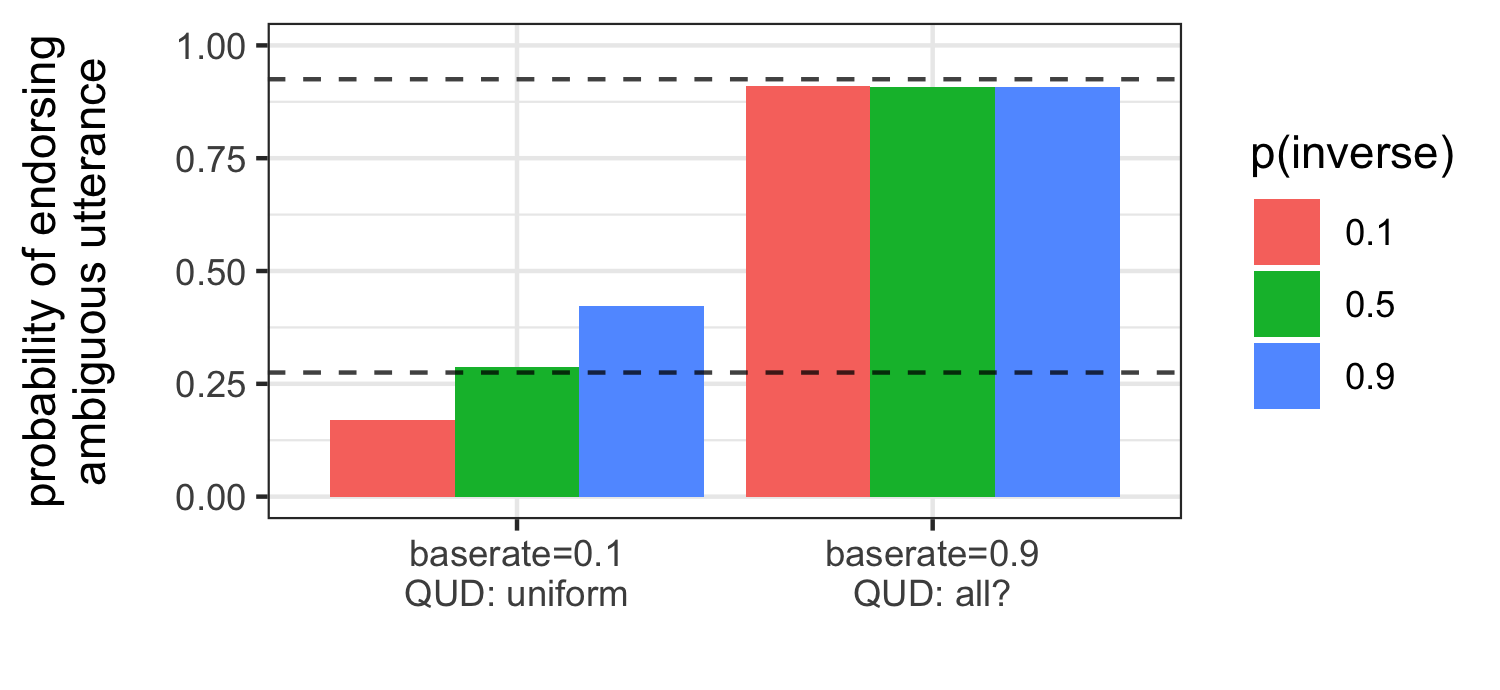
\includegraphics[height=1.55in]{two-not-pragmatic.png}
% \vspace{-20pt}
\caption{Model predictions for ambiguous \textit{two-not} utterance endorsement in a \textsc{1-of-2} context when multiple factors interact. Dashed lines represent experimentally-observed endorsement behavior in the absence (lower) vs.~presence (upper) of an explicit contrast}
\label{fig:interactions}
% \vspace{-10pt}
\end{figure}

The right side of Figure 
\ref{fig:interactions} replicates Figure \ref{fig:interaction}: 
\lp{we see that access to the inverse scope has very little impact on the endorsement rate.}
%, which is at XYX (0.87?) when the baserate $b_{suc}$ is 0.9 and the QUD \texttt{all?} prior is also 0.9.}
\lp{This contrasts with the left side of Figure \ref{fig:interactions},
 where a low baserate ($b_{suc}$=0.1) and a uniform prior on QUDs (so \texttt{all?}~isn't favored) lead 
% On  %in that case, 
access to the inverse scope to have a noticeable effect}, with endorsement increasing with the prior probability of the \texttt{inverse} interpretation. 
%, increasing endorsement rates from XYX (0.18?) to XYX (0.41?).
% Importantly, when it's just as easy to access the inverse scope as the surface scope (the scope prior = 0.5), but the pragmatic context isn't as supportive ($b_{suc}$=0.1; uniform prior on QUDs), we see a predicted endorsement rate around XYX (0.27?). 
%This predicted rate is near the empirically-observed rate of 27.5\% in the context without the early-success explicit contrast.
%}
Given these predictions, \lp{it seems that} the empirically-observed low-endorsement baseline (27.5\%) most likely results from low expectations for success ($b_{suc}=0.1$) and QUD uncertainty (QUD: \texttt{uniform}), together with a moderate-to-low probability of accessing the \texttt{inverse} scope ($P(inv)=0.1$ or $0.5$). From this baseline, we \lp{can} implement the effect of the explicit contrast manipulation by increasing success expectations ($b_{suc}=0.9$) and shifting the topic of conversation to whether total success occurred (QUD: \texttt{all?}). This manipulation results in a dramatic increase in utterance endorsement, irrespective of scope. 

To summarize, if the explicit contrast clause impacts a listener's beliefs about the horses' chance of success (increasing $b_{suc}$) or the QUD (favoring \texttt{all?}), then the model predicts the endorsement rate should increase. Notably, both of these manipulations make the \emph{two-not} scopally-ambiguous utterance more informative for a listener. In the case of the the world state manipulation, \emph{two-not}---under either scope interpretation---informs the listener that her prior beliefs about total horse success do not hold. Similarly with the QUD manipulation favoring \texttt{all?}, both scope interpretations answer this question in the negative (i.e., it is not the case that all (two) horses succeeded). 


\subsubsection{The \textsc{1-of-2} vs.~\textsc{2-of-4} asymmetry}

\lp{Our model predicts that these factors should be active in utterance disambiguation more generally; therefore, the same model implementation used to capture \textsc{1-of-2} endorsement behavior should be able to capture \textsc{2-of-4} endorsement behavior.}
\lp{More specifically,}
we would expect the very same factors and values to additionally capture the high endorsement rate in the \textsc{2-of-4} context \lp{\emph{without}} the explicit contrast. 
If \lp{so, we would have computational modeling evidence that}
the factors identified for capturing the experimentally-observed effect of the explicit contrast are indeed active in utterance disambiguation \lp{more generally.} 
%(i.e., to validate their explanatory power), 



Recall the baseline \textsc{1-of-2} parameter values most likely to lead to low endorsement: low expectations for success ($b_{suc}=0.1$) and QUD uncertainty (QUD: \texttt{uniform}). To model the \textsc{2-of-4} context, we change the number of actors $n$ to 4 and additionally manipulate whether the {exact} ($=$) or {at-least} ($\geq$) utterance semantics applies, as predictions diverge when there are more than two actors in the context (recall the discussion in Section \ref{two-model-specification}). This decision impacts both the utterance semantics and the relevant set of QUDs (e.g., if the at-least semantics gets used, then the $\texttt{two}_{\geq}\texttt{?}$~QUD is included in the set of potential QUDs). 

As shown in Figure \ref{fig:2of4}, we do indeed predict high endorsement with the same parameter value baseline, but only with {exact} utterance semantics and a 
%moderate to 
\lp{fairly}
low probability of accessing the inverse scope ($P(inv)$ = 0.1).
\lp{This prediction is shown on the right side of Figure \ref{fig:2of4}, where a high endorsement rate is predicted with the pragmatic factors identified above ($b_{suc}=0.1$, QUD prior is uniform), as long as 
%access to the inverse scope is fairly low ($P(inv)$ = 0.1) and 
the numeral \textit{two} has an exact semantics and access to \texttt{inverse} scope is low ($P(inv)$ $<$ 0.5).
In contrast, when \textit{two} has an at-least semantics (left side of Figure 4), the model predicts low endorsement with} these pragmatic factors.

\begin{figure}[!ht]
\centering
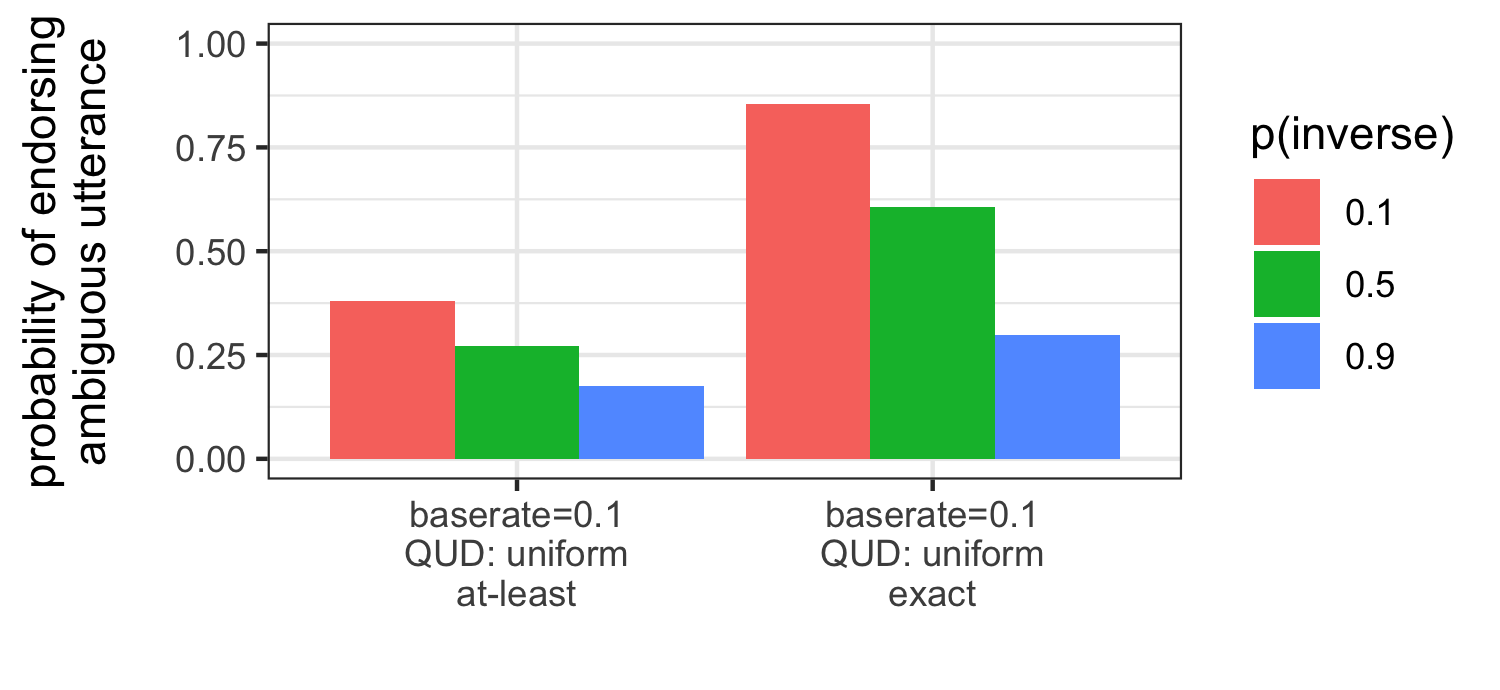
\includegraphics[height=1.55in]{two-not-four.png}
% \vspace{-20pt}
\caption{Model predictions for ambiguous \textit{two-not} endorsement in a \textsc{2-of-4} \lp{context} with a low baserate of success is low (0.1) and QUD uncertainty (uniform QUD prior). On the left, we see predictions for an at-least semantics; on the right, we see predictions for an exact semantics}
\label{fig:2of4}
% \vspace{-10pt}
\end{figure}

\subsection{Discussion}

Our model of \emph{two-not} utterances---a straightforward extension of the \emph{every-not} model---captures the effect of the early-success explicit-contrast manipulation observed in adults. Notably, we saw that the \emph{every-not} model captures the same effect in children. This parallelism---sensitivity to the pragmatic context in both children and adults across different contexts---suggests that the same disambiguation mechanism is active in both children and adults. Adults seem better able to charitably interpret less-supportive pragmatic contexts (i.e., the original \emph{every-not} scenarios); 
% , \lp{certain \textit{two-not} contexts, like the 2-of-4 scenario}); \gcs{I wouldn't call these contexts less supportive}
yet, there remain scenarios (i.e., the \textsc{1-of-2} \emph{two-not} contexts) %\lp{like the 1-of-2 scenario}) 
where even adult abilities are exceeded. We interpret the common underlying mechanism as support for developmental continuity in scope ambiguity resolution;
no qualitative shift \lp{is} required \lp{for five-year-old children to become adult-like in how they resolve scope ambiguity in context}.

% In addition to supporting the developmental continuity hypothesis, this model also suggests {why} manipulations like the explicit contrast clause work. The pragmatic variables capture the explicit contrast manipulation because they create a situation where the ambiguous \emph{two-not} utterance is still informative {despite} the ambiguity. When the utterance provides the listener with information that diverges from her prior beliefs, the ambiguous \textit{two-not} utterance becomes more informative, more useful, and therefore more endorsable. 

The model also captures \citeauthor{musolinolidz2003}'s results from the \textsc{2-of-4} context: with the very same parameter values that yield low endorsement rates for \textsc{1-of-2} contexts, the model predicts the high endorsement observed for \textsc{2-of-4} contexts. The only change is increasing the number of relevant individuals from two to four. This exploration of the \textsc{1-of-2} vs.~\textsc{2-of-4} contexts allows us to refine our understanding of the potential sources of child and adult behavior. Our findings from the \emph{every-not} model suggested that pragmatic factors alone are capable of capturing the non-adult-like behavior in children, and the extension in the current model captures the explicit-contrast effect in adults; however, it appears that the processing factor of scope access (in particular, disfavoring the inverse scope) is needed to account for \citeauthor{musolinolidz2003}'s \lp{adult} \textsc{2-of-4} results. This finding supports the conclusion of \citeauthor{musolinolidz2003}, namely that adults have a strong preference for surface interpretations of \emph{two-not} utterances. Combined with the appropriate pragmatic context, that preference has the potential to drive the endorsement asymmetry between the \textsc{1-of-2} and \textsc{2-of-4} contexts. Whether this surface-interpretation preference for  \textit{two-not} utterances is also something children share remains an open empirical question; experimental results for \emph{every-not} do not answer this question definitively \citep{viauetal2010}.

\lp{Interestingly}, the current model requires one more ingredient to account for the \textsc{1-of-2} vs.~\textsc{2-of-4} difference in adult behavior: an {exact} semantics for utterances with numerals (in contrast to an {at-least} semantics; cf.~\citealp{geurts2006,breheny2008,spector2013,kennedy2015}). While the underlying utterance semantics is not something easy to manipulate in an experiment, it is exactly the kind of variable we can systematically explore in a computational \lp{cognitive} model. By doing so here, we are able to show the necessity of an {exact} semantics in generating observable adult behavior. This result provides empirical support, coming from computational \lp{cognitive} modeling, for theories about the semantics and pragmatics of numerals. In particular, we account for the observed adult behavior by assuming that adults interpret \textit{two} utterances as meaning {exactly} two \lp{and not at least two}.




\section{General discussion} \label{discussion}
Truth-value judgments 
% \lp{(truth-value judgments)}
serve a critical role in diagnostics of linguistic meaning, yet the cognitive processes involved in generating these judgments\lp{---particularly the precise impact of context on pragmatic reasoning---}\lp{have rarely been formally} examined. Here, we have 
% brought a critical eye 
\lp{formally investigated the cognitive underpinnings of the}
%to the 
%truth-value judgment 
\lp{truth-value judgment}
methodology. We used as our case study the phenomenon of scope ambiguity, where children's behavior often deviates noticeably from that of adults; yet, \lp{both child and adult behavior can be} profoundly affected by changes to task setups.  Using the methodology of computational cognitive modeling, we advanced precise hypotheses about how linguistic knowledge, world knowledge, and general social reasoning interact to deliver observed behavior in the 
\lp{truth-value judgment}
%truth-value judgment 
task.

Our model of utterance endorsement in the %truth-value judgment 
\lp{truth-value judgment}
task predicts the lowest rates of utterance endorsement for ambiguous utterances in not-all  scenarios (as in Figure \ref{not-all})
% \lp{(like {1-of-2} horses jumping over a fence)}
when neither interpretation---surface or inverse---is useful for successful communication.
\lp{The interpretation could be less useful}
 because the interpretation is false;  
\lp{for example, the surface interpretation \emph{every-not} is false in the not-all scenario.}
\lp{The interpretation could also be less useful} 
because beliefs about the pragmatic context render the interpretation uninformative;
\lp{for example, if we 
% b_suc = 0.1
expect horses should be unsuccessful at jumping 
or 
% uniform prior on QUD
we are uncertain about the conversational topic in a not-all scenario,
% so saying not all the horses were successful is imprecise
the inverse interpretation of \emph{every-not} %\textit{Not all the horses jumped} 
is frustratingly imprecise.
} 
\lp{Given} these observations, 
 the utterance non-endorsement \lp{behavior} \lp{that has been} previously used to demonstrate children's difficulty with {inverse} scope calculation in fact requires no disambiguation at all if the goal is informative communication \lp{(as mentioned above, both interpretations can be uninformative in certain pragmatic contexts)}. Instead, children (and adults) simply need the ability to manage the pragmatic context so they can recognize the potential informativity of these ambiguous utterances. Notably, considerations of pragmatic context have long played a role in the design and interpretation of the 
 %truth-value judgment 
 \lp{truth-value judgment}
 task (e.g., \citealp{crainetal1996}). Here we have taken the extra step of formally articulating specific pragmatic factors and the role they play in children's apparent difficulty with ambiguous utterances in the
 \lp{truth-value judgment}
 %truth-value judgment 
 task.
 \lp{In this way, we can specify how changing the experimental context impacts the pragmatic factors that underlie children's truth-value judgment endorsement behavior.}

We saw that two aspects of the pragmatic context have an outsized effect on utterance endorsement, and for similar reasons. When the QUD is such that the ambiguous utterance provides a full answer under either scope interpretation, we recognize the ambiguous utterance as a useful thing to say, and so participants are more likely to endorse it as a communicative act. 
\lp{For example, in a not-all horse-jumping scenario, if we care about whether all of the horses jumped, either interpretation is useful---both the surface %\textit{None of the horses jumped} 
and the inverse %\textit{Not all of the horses jumped} 
interpretations tell us that the answer is ``no''.}
When prior beliefs about the world context and what counts as a likely state of affairs are contradicted by the ambiguous utterance---again, under either scope interpretation---the utterance is potentially very informative, which makes it more useful and thus more likely to be endorsed. 
\lp{For example, in a not-all scenario, if we think horses nearly always succeed in jumping, we would expect the world where all the horses are successful to be most likely; here, either interpretation is useful because both the surface %\textit{None of the horses jumped} 
and the inverse %\textit{Not all of the horses jumped} 
interpretations
tell us that the world where all the horses are successful is in fact not the one we are in.}

\lp{So,} in order to endorse the \lp{ambiguous} utterance, a \lp{truth-value judgment} experimental participant must be able to manage the pragmatic context in such a way that allows them to recognize the potential utility of the ambiguous utterance. With \emph{every-not} utterances, adults are able to manage the pragmatic context in this way, while children require additional support. And with \emph{two-not} utterances, even adults require additional support to manage the pragmatic context \lp{in certain scenarios}.

Our findings underscore the complexity of information involved in interpreting scopally-ambiguous utterances, including the literal semantics of the utterances involved, processing factors that affect interpretation accessibility, pragmatic factors that affect the potential informativity of the utterance, and the recursive social reasoning between speakers and listeners. Over the course of two applications---explaining children's non-adult-like behavior with \emph{every-not} utterances and adults' child-like behavior with \emph{two-not} utterances---we find evidence for the impact of both pragmatic and processing factors on 
\lp{truth-value judgment}
%truth-value judgment 
behavior; \lp{in particular,} \lp{we see} how a specific confluence of values for these factors yields the observed utterance endorsement behavior in multiple contexts. The fact that the same pragmatic factors can have such a pronounced effect on both child and adult behavior highlights the developmental continuity in pragmatic reasoning from childhood to adulthood. Moreover, the fact that the processing factor of scope access is crucial for explaining adult behavior in certain contexts motivates experimental work with children to see if their behavior is likewise affected by this processing factor in similar contexts. 

% The fact that only the \texttt{exact} utterance semantics is capable of yielding the observed behavior provides empirical support in favor of this theory of representation for numerals. 

More broadly, we have demonstrated how computational \lp{cognitive} modeling can help us refine our theories about different aspects of language, including theories of language understanding, language development, and language representation. Importantly, we have shown how analytic results allow for a better understanding of behavior in the 
%truth-value judgment 
\lp{truth-value judgment}
task, thereby allowing for a better understanding of the task itself and thus a cleaner mapping between our \lp{cognitive} theories \lp{of ambiguity resolution}  and the data that test them. The moral is as follows: before we can \lp{effectively interpret} 
%truth-value judgment
\lp{truth-value judgment}
behavior \lp{with respect to our theories of processing, development, and representation}, we must understand the pragmatics involved; the current work offers a path toward that understanding. 

% understanding task behavior promises to inform our understanding of the task itself, thereby allowing for a cleaner mapping between our theories and the data that test them.

% \section{Conclusion} \label{conclusion}



%\newpage

% \section*{References}

% \bibliographystyle{chicago}
\bibliography{bibliography}

\end{document}